\PassOptionsToPackage{unicode=true}{hyperref} % options for packages loaded elsewhere
\PassOptionsToPackage{hyphens}{url}
\PassOptionsToPackage{dvipsnames,svgnames*,x11names*}{xcolor}
%
\documentclass[12pt,]{book}
\usepackage{lmodern}
\usepackage{amssymb,amsmath}
\usepackage{ifxetex,ifluatex}
\usepackage{fixltx2e} % provides \textsubscript
\ifnum 0\ifxetex 1\fi\ifluatex 1\fi=0 % if pdftex
  \usepackage[T1]{fontenc}
  \usepackage[utf8]{inputenc}
  \usepackage{textcomp} % provides euro and other symbols
\else % if luatex or xelatex
  \usepackage{unicode-math}
  \defaultfontfeatures{Ligatures=TeX,Scale=MatchLowercase}
\fi
% use upquote if available, for straight quotes in verbatim environments
\IfFileExists{upquote.sty}{\usepackage{upquote}}{}
% use microtype if available
\IfFileExists{microtype.sty}{%
\usepackage[]{microtype}
\UseMicrotypeSet[protrusion]{basicmath} % disable protrusion for tt fonts
}{}
\IfFileExists{parskip.sty}{%
\usepackage{parskip}
}{% else
\setlength{\parindent}{0pt}
\setlength{\parskip}{6pt plus 2pt minus 1pt}
}
\usepackage{xcolor}
\usepackage{hyperref}
\hypersetup{
            pdftitle={PRIORITIZR WORKSHOP MANUAL},
            pdfauthor={Jeffrey O. Hanson},
            colorlinks=true,
            linkcolor=Maroon,
            filecolor=Maroon,
            citecolor=Blue,
            urlcolor=blue,
            breaklinks=true}
\urlstyle{same}  % don't use monospace font for urls
\usepackage[left=2.54cm, right=2.54cm, top=2.54cm, bottom=2.54cm]{geometry}
\usepackage{color}
\usepackage{fancyvrb}
\newcommand{\VerbBar}{|}
\newcommand{\VERB}{\Verb[commandchars=\\\{\}]}
\DefineVerbatimEnvironment{Highlighting}{Verbatim}{commandchars=\\\{\}}
% Add ',fontsize=\small' for more characters per line
\usepackage{framed}
\definecolor{shadecolor}{RGB}{248,248,248}
\newenvironment{Shaded}{\begin{snugshade}}{\end{snugshade}}
\newcommand{\AlertTok}[1]{\textcolor[rgb]{0.94,0.16,0.16}{#1}}
\newcommand{\AnnotationTok}[1]{\textcolor[rgb]{0.56,0.35,0.01}{\textbf{\textit{#1}}}}
\newcommand{\AttributeTok}[1]{\textcolor[rgb]{0.77,0.63,0.00}{#1}}
\newcommand{\BaseNTok}[1]{\textcolor[rgb]{0.00,0.00,0.81}{#1}}
\newcommand{\BuiltInTok}[1]{#1}
\newcommand{\CharTok}[1]{\textcolor[rgb]{0.31,0.60,0.02}{#1}}
\newcommand{\CommentTok}[1]{\textcolor[rgb]{0.56,0.35,0.01}{\textit{#1}}}
\newcommand{\CommentVarTok}[1]{\textcolor[rgb]{0.56,0.35,0.01}{\textbf{\textit{#1}}}}
\newcommand{\ConstantTok}[1]{\textcolor[rgb]{0.00,0.00,0.00}{#1}}
\newcommand{\ControlFlowTok}[1]{\textcolor[rgb]{0.13,0.29,0.53}{\textbf{#1}}}
\newcommand{\DataTypeTok}[1]{\textcolor[rgb]{0.13,0.29,0.53}{#1}}
\newcommand{\DecValTok}[1]{\textcolor[rgb]{0.00,0.00,0.81}{#1}}
\newcommand{\DocumentationTok}[1]{\textcolor[rgb]{0.56,0.35,0.01}{\textbf{\textit{#1}}}}
\newcommand{\ErrorTok}[1]{\textcolor[rgb]{0.64,0.00,0.00}{\textbf{#1}}}
\newcommand{\ExtensionTok}[1]{#1}
\newcommand{\FloatTok}[1]{\textcolor[rgb]{0.00,0.00,0.81}{#1}}
\newcommand{\FunctionTok}[1]{\textcolor[rgb]{0.00,0.00,0.00}{#1}}
\newcommand{\ImportTok}[1]{#1}
\newcommand{\InformationTok}[1]{\textcolor[rgb]{0.56,0.35,0.01}{\textbf{\textit{#1}}}}
\newcommand{\KeywordTok}[1]{\textcolor[rgb]{0.13,0.29,0.53}{\textbf{#1}}}
\newcommand{\NormalTok}[1]{#1}
\newcommand{\OperatorTok}[1]{\textcolor[rgb]{0.81,0.36,0.00}{\textbf{#1}}}
\newcommand{\OtherTok}[1]{\textcolor[rgb]{0.56,0.35,0.01}{#1}}
\newcommand{\PreprocessorTok}[1]{\textcolor[rgb]{0.56,0.35,0.01}{\textit{#1}}}
\newcommand{\RegionMarkerTok}[1]{#1}
\newcommand{\SpecialCharTok}[1]{\textcolor[rgb]{0.00,0.00,0.00}{#1}}
\newcommand{\SpecialStringTok}[1]{\textcolor[rgb]{0.31,0.60,0.02}{#1}}
\newcommand{\StringTok}[1]{\textcolor[rgb]{0.31,0.60,0.02}{#1}}
\newcommand{\VariableTok}[1]{\textcolor[rgb]{0.00,0.00,0.00}{#1}}
\newcommand{\VerbatimStringTok}[1]{\textcolor[rgb]{0.31,0.60,0.02}{#1}}
\newcommand{\WarningTok}[1]{\textcolor[rgb]{0.56,0.35,0.01}{\textbf{\textit{#1}}}}
\usepackage{longtable,booktabs}
% Fix footnotes in tables (requires footnote package)
\IfFileExists{footnote.sty}{\usepackage{footnote}\makesavenoteenv{longtable}}{}
\usepackage{graphicx,grffile}
\makeatletter
\def\maxwidth{\ifdim\Gin@nat@width>\linewidth\linewidth\else\Gin@nat@width\fi}
\def\maxheight{\ifdim\Gin@nat@height>\textheight\textheight\else\Gin@nat@height\fi}
\makeatother
% Scale images if necessary, so that they will not overflow the page
% margins by default, and it is still possible to overwrite the defaults
% using explicit options in \includegraphics[width, height, ...]{}
\setkeys{Gin}{width=\maxwidth,height=\maxheight,keepaspectratio}
\setlength{\emergencystretch}{3em}  % prevent overfull lines
\providecommand{\tightlist}{%
  \setlength{\itemsep}{0pt}\setlength{\parskip}{0pt}}
\setcounter{secnumdepth}{5}
% Redefines (sub)paragraphs to behave more like sections
\ifx\paragraph\undefined\else
\let\oldparagraph\paragraph
\renewcommand{\paragraph}[1]{\oldparagraph{#1}\mbox{}}
\fi
\ifx\subparagraph\undefined\else
\let\oldsubparagraph\subparagraph
\renewcommand{\subparagraph}[1]{\oldsubparagraph{#1}\mbox{}}
\fi

% set default figure placement to htbp
\makeatletter
\def\fps@figure{htbp}
\makeatother

% load packages
\usepackage{caption}
\usepackage{float}

% default bookdown preamble
\usepackage{booktabs}
\usepackage{amsthm}
\makeatletter
\def\thm@space@setup{%
  \thm@preskip=8pt plus 2pt minus 4pt
  \thm@postskip=\thm@preskip
}
\makeatother

% remove figure labelling
\captionsetup[figure]{labelformat=empty,textfont=it}

% make figures static
\let\origfigure\figure
\let\endorigfigure\endfigure
\renewenvironment{figure}[1][2] {
  \expandafter\origfigure\expandafter[H]
} {
  \endorigfigure
}

% text boxes
\ifxetex
  \usepackage{letltxmacro}
  \setlength{\XeTeXLinkMargin}{1pt}
  \LetLtxMacro\SavedIncludeGraphics\includegraphics
  \def\includegraphics#1#{% #1 catches optional stuff (star/opt. arg.)
    \IncludeGraphicsAux{#1}%
  }%
  \newcommand*{\IncludeGraphicsAux}[2]{%
    \XeTeXLinkBox{%
      \SavedIncludeGraphics#1{#2}%
    }%
  }%
\fi

\makeatletter
\newenvironment{kframe}{%
\medskip{}
\setlength{\fboxsep}{.8em}
 \def\at@end@of@kframe{}%
 \ifinner\ifhmode%
  \def\at@end@of@kframe{\end{minipage}}%
  \begin{minipage}{\columnwidth}%
 \fi\fi%
 \def\FrameCommand##1{\hskip\@totalleftmargin \hskip-\fboxsep
 \colorbox{shadecolor}{##1}\hskip-\fboxsep
     % There is no \\@totalrightmargin, so:
     \hskip-\linewidth \hskip-\@totalleftmargin \hskip\columnwidth}%
 \MakeFramed {\advance\hsize-\width
   \@totalleftmargin\z@ \linewidth\hsize
   \@setminipage}}%
 {\par\unskip\endMakeFramed%
 \at@end@of@kframe}
\makeatother

\makeatletter
\@ifundefined{Shaded}{
}{\renewenvironment{Shaded}{\begin{kframe}}{\end{kframe}}}
\makeatother

\newenvironment{rmdblock}[1]
  {
  \begin{itemize}
  \renewcommand{\labelitemi}{
    \raisebox{-.7\height}[0pt][0pt]{
      {\setkeys{Gin}{width=3em,keepaspectratio}\includegraphics{images/#1}}
    }
  }
  \setlength{\fboxsep}{1em}
  \begin{kframe}
  \item
  }
  {
  \end{kframe}
  \end{itemize}
  }
\newenvironment{rmdnote}
  {\begin{rmdblock}{note}}
  {\end{rmdblock}}
\newenvironment{rmdcaution}
  {\begin{rmdblock}{caution}}
  {\end{rmdblock}}
\newenvironment{rmdquestion}
  {\begin{rmdblock}{question}}
  {\end{rmdblock}}
\newenvironment{rmdanswer}
  {\begin{rmdblock}{answer}}
  {\end{rmdblock}}
\newenvironment{rmdimportant}
  {\begin{rmdblock}{important}}
  {\end{rmdblock}}
\newenvironment{rmdtip}
  {\begin{rmdblock}{tip}}
  {\end{rmdblock}}
\newenvironment{rmdwarning}
  {\begin{rmdblock}{warning}}
  {\end{rmdblock}}
\usepackage[]{natbib}
\bibliographystyle{plainnat}

\title{PRIORITIZR WORKSHOP MANUAL}
\author{Jeffrey O. Hanson}
\date{2023-03-29}

\begin{document}
\maketitle

{
\hypersetup{linkcolor=}
\setcounter{tocdepth}{0}
\tableofcontents
}
\hypertarget{welcome}{%
\chapter{Welcome!}\label{welcome}}

Here you will find the manual for the prioritizr module of the \href{https://prioritizr.github.io/NCC-workshop/}{Automation \& Technical Skills GIS Group Meeting}. \textbf{Before you arrive at the workshop, you should make sure that you have correctly \protect\hyperlink{setup}{set up your computer for the workshop} and you have \href{https://github.com/prioritizr/NCC-workshop/raw/main/data.zip}{downloaded the data from here}.}

\hypertarget{introduction}{%
\chapter{Introduction}\label{introduction}}

\hypertarget{overview}{%
\section{Overview}\label{overview}}

The aim of this workshop is to help you get started with using the prioritizr R package for systematic conservation planning. It is not designed to give you a comprehensive overview and you will not become an expert after completing this workshop. Instead, we want to help you understand the core principles of conservation planning and guide you through some of the common tasks involved with developing prioritizations. In other words, we want to give you the knowledge base and confidence needed to start applying systematic conservation planning to your own work.

You are not alone in this workshop. If you are having trouble, please put your hand up and one of the instructors will help you as soon as they can. You can also ask the people sitting next to you for help too. \textbf{Most importantly, the code needed to answer the questions in this workshop are almost always located in the same section as the question. So if you are stuck, try rereading the example code and see if you can modify it to answer the question.} Please note that the first thing an instructor will ask you will be ``what have you tried so far?''. We can't help you if you haven't tried anything.

\hypertarget{setup}{%
\section{Setting up your computer}\label{setup}}

You will need to have both \href{https://www.r-project.org}{R} and \href{https://www.rstudio.com/}{RStudio} installed on your computer to complete this workshop. Although it is not imperative that you have the latest version of RStudio installed, \textbf{you will need the latest version of R installed (i.e.~version 4.2.3)}. Please note that you might need administrative permissions to install these programs. After installing them, you will also need to install some R packages too.

\hypertarget{r}{%
\subsection{R}\label{r}}

The \href{https://www.r-project.org}{R statistical computing environment} can be downloaded from the Comprehensive R Archive Network (CRAN). Specifically, you can download the latest version of R (version 4.2.3) from here: \url{https://cloud.r-project.org}. Please note that you will need to download the correct file for your operating system (i.e.~Linux, Mac OSX, Windows).

\hypertarget{rstudio}{%
\subsection{RStudio}\label{rstudio}}

\href{https://www.rstudio.com}{RStudio} is an integrated development environment (IDE). In other words, it is a program that is designed to make your R programming experience more enjoyable. During this workshop, you will interact with R through RStudio---meaning that you will open RStudio to code in R. You can download the latest version of RStudio here: \url{http://www.rstudio.com/download}. When you start RStudio, you will see two main parts of the interface:

\begin{center}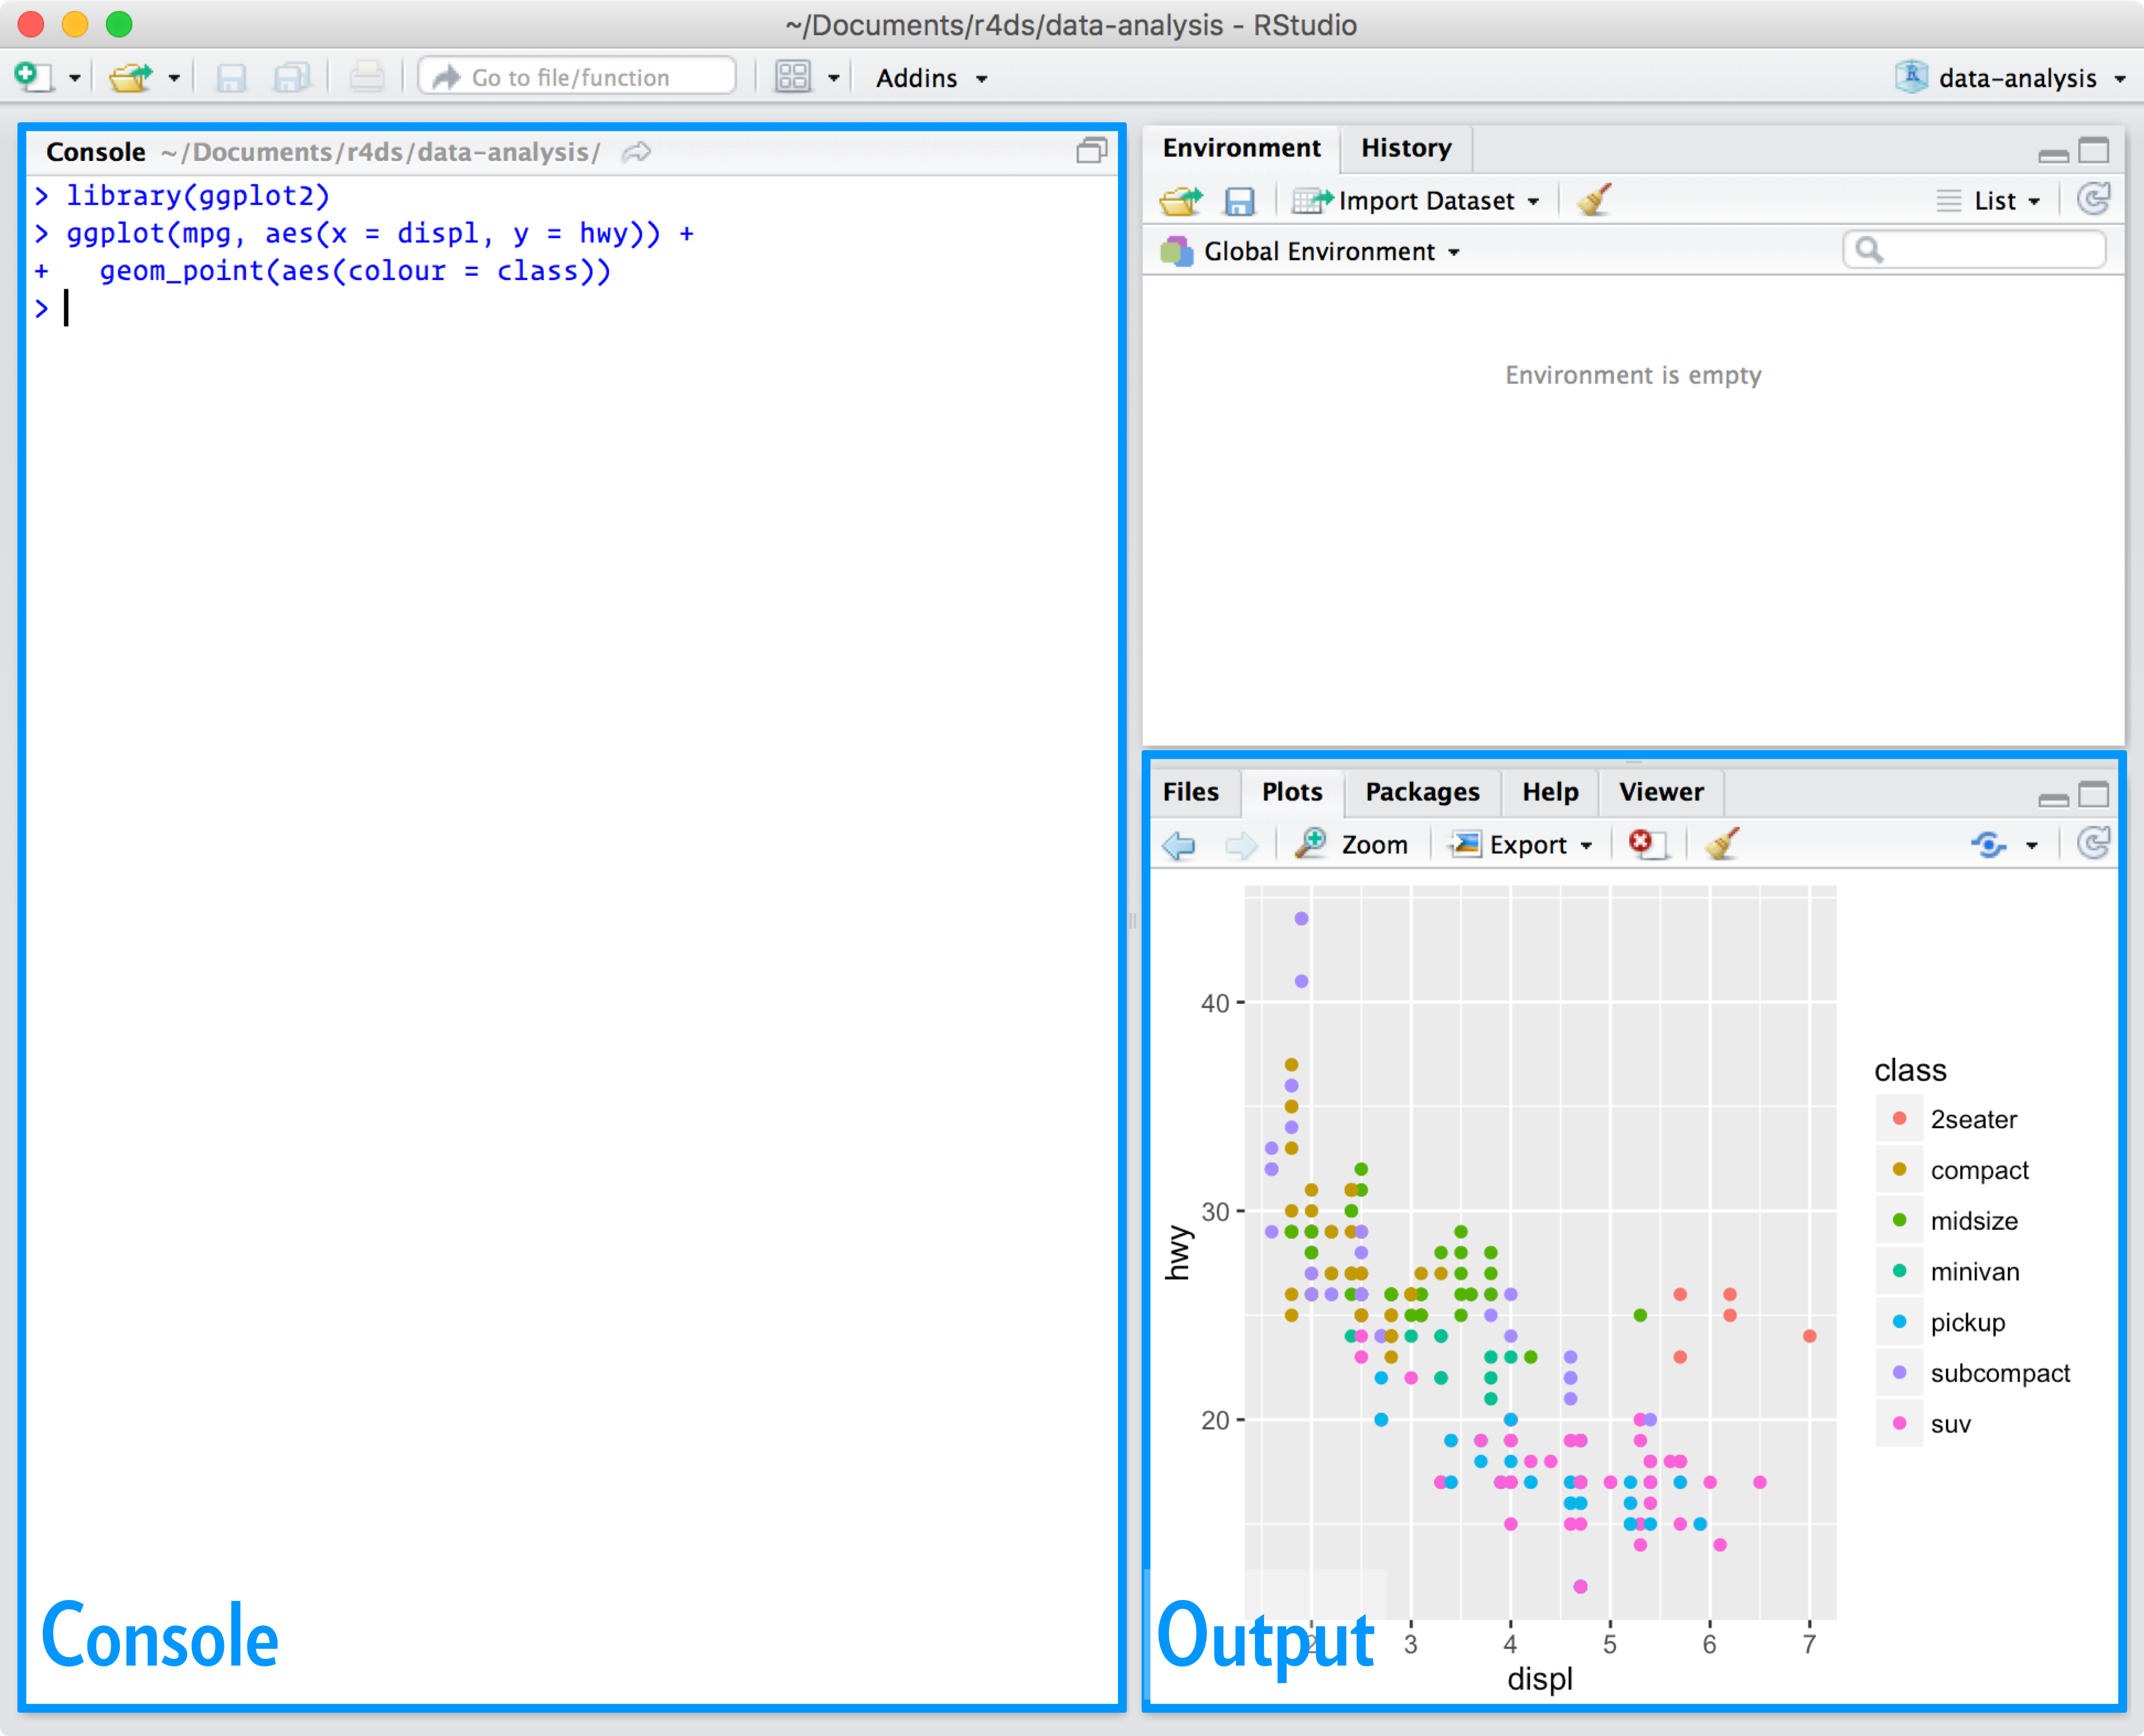
\includegraphics[width=1\linewidth]{images/rstudio-console} \end{center}

You can type R code into the \emph{Console} and press the enter key to run code.

\hypertarget{r-packages}{%
\subsection{R packages}\label{r-packages}}

An R package is a collection of R code and documentation that can be installed to enhance the standard R environment with additional functionality. Currently, there are over fifteen thousand R packages available on CRAN. Each of these R packages are developed to perform a specific task, such as \href{https://cran.r-project.org/web/packages/readxl/index.html}{reading Excel spreadsheets}, \href{https://cran.r-project.org/web/packages/MODIStsp/index.html}{downloading satellite imagery data}, \href{https://cran.r-project.org/web/packages/wdpar/index.html}{downloading and cleaning protected area data}, or \href{https://cran.r-project.org/web/packages/ENMeval/index.html}{fitting environmental niche models}. In fact, R has such a diverse ecosystem of R packages, that the question is almost always not ``can I use R to \ldots{}?'' but ``what R package can I use to \ldots{}?''. During this workshop, we will use several R packages. To install these R packages, please enter the code below in the \emph{Console} part of the RStudio interface and press enter. Note that you will require an Internet connection and the installation process may take some time to complete.

\begin{Shaded}
\begin{Highlighting}[]
\KeywordTok{install.packages}\NormalTok{(}\KeywordTok{c}\NormalTok{(}\StringTok{"sf"}\NormalTok{, }\StringTok{"tidyverse"}\NormalTok{, }\StringTok{"sp"}\NormalTok{, }\StringTok{"rgeos"}\NormalTok{, }\StringTok{"rgdal"}\NormalTok{, }\StringTok{"raster"}\NormalTok{,}
                   \StringTok{"units"}\NormalTok{, }\StringTok{"prioritizr"}\NormalTok{, }\StringTok{"prioritizrdata"}\NormalTok{, }\StringTok{"Rsymphony"}\NormalTok{,}
                   \StringTok{"mapview"}\NormalTok{, }\StringTok{"assertthat"}\NormalTok{, }\StringTok{"velox"}\NormalTok{, }\StringTok{"remotes"}\NormalTok{,}
                   \StringTok{"gridExtra"}\NormalTok{))}

\ControlFlowTok{if}\NormalTok{ (}\OperatorTok{!}\KeywordTok{require}\NormalTok{(remotes)) }\KeywordTok{install.packages}\NormalTok{(}\StringTok{"remotes"}\NormalTok{)}
\NormalTok{remotes}\OperatorTok{::}\KeywordTok{install_bioc}\NormalTok{(}\StringTok{"lpsymphony"}\NormalTok{)}
\end{Highlighting}
\end{Shaded}

\hypertarget{further-reading}{%
\section{Further reading}\label{further-reading}}

There is a wealth of resources available for learning how to use R. Although not required for this workshop, I would highly recommend that you read \href{https://r4ds.had.co.nz/}{\emph{R for Data Science} by Garrett Grolemund and Hadley Wickham}. \textbf{This veritable trove of R goodness is freely available online.} If you spend a week going through this book then you will save months debugging and rerunning incorrect code. I would urge any and all ecologists, especially those working on Masters or PhD degrees, to read this book. I even bought this book as a Christmas present for my sister---and, yes, she was happy to receive it! For intermediate users looking to skill-up, I would recommend the \href{http://shop.oreilly.com/product/9781593273842.do}{\emph{The Art of R Programming: A Tour of Statistical Software Design} by Norman Matloff} and \href{https://adv-r.hadley.nz/}{\emph{Advanced R} by Hadley Wickham}. Finally, if you wish to learn more about using R as a geospatial information system (GIS), I would recommend \href{https://geocompr.robinlovelace.net/}{\emph{Geocomputation with R} by Robin Lovelace, Jakub Nowosad, and Jannes Muenchow} which is also freely available online. I also recommend \href{https://www.springer.com/gp/book/9781461476177}{\emph{Applied Spatial Data Analysis} by Roger S. Bivand, Edzer Pebesma, and Virgilio Gómez-Rubio} too.

\hypertarget{data}{%
\chapter{Data}\label{data}}

\hypertarget{starting-out}{%
\section{Starting out}\label{starting-out}}

We will start by opening RStudio. Ideally, you will have already installed both R and Rstudio before the workshop. If you have not done this already, then please see the \protect\hyperlink{setup}{Setting up your computer} section. \textbf{During this workshop, please do not copy and paste code from the workshop manual into RStudio. Instead, please write it out yourself in an R script.} When programming, you will spend a lot of time fixing coding mistakes---that is, debugging your code---so it is best to get used to making mistakes now when you have people here to help you. You can create a new R script by clicking on \emph{File} in the RStudio menu bar, then \emph{New File}, and then \emph{R Script}.

\begin{center}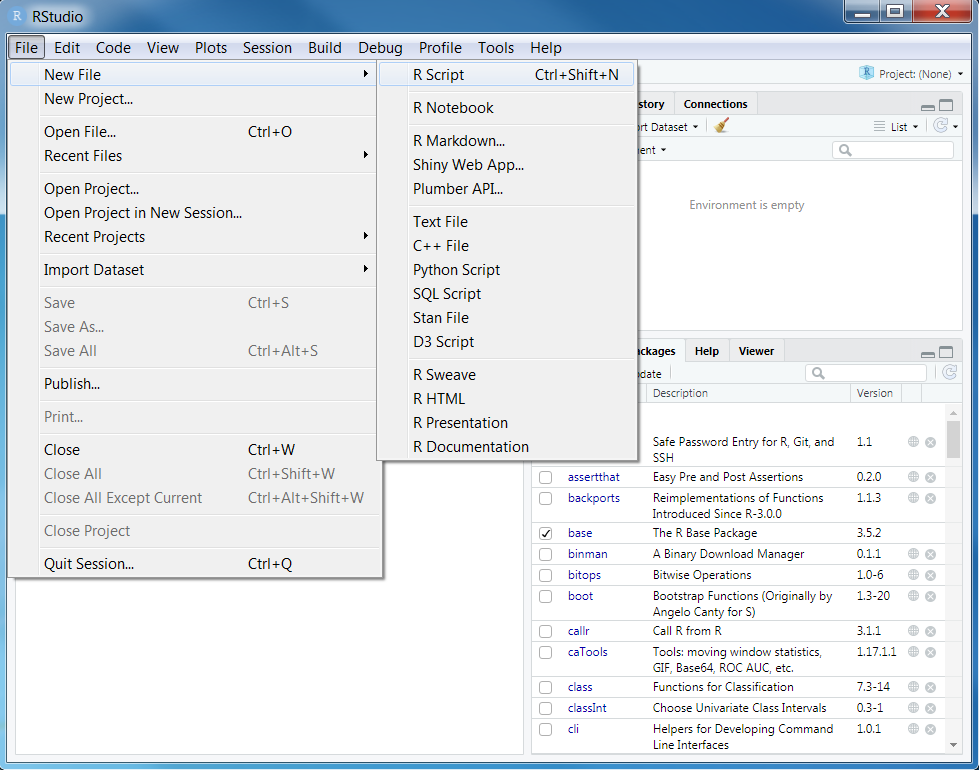
\includegraphics[width=0.7\linewidth]{images/rstudio-new-script} \end{center}

After creating a new script, you will notice that a new \emph{Source} panel has appeared. In the \emph{Source} panel, you can type and edit code before you run it. You can run code in the \emph{Source} panel by placing the cursor (i.e.~the blinking line) on the desired line of code and pressing \texttt{Control\ +\ Enter} on your keyboard (or \texttt{CMD\ +\ Enter} if you are using an Apple computer). You can save the code in the \emph{Source} panel by pressing \texttt{Control\ +\ s} on your keyboard (or \texttt{CMD\ +\ s} if you are using an Apple computer).

\begin{center}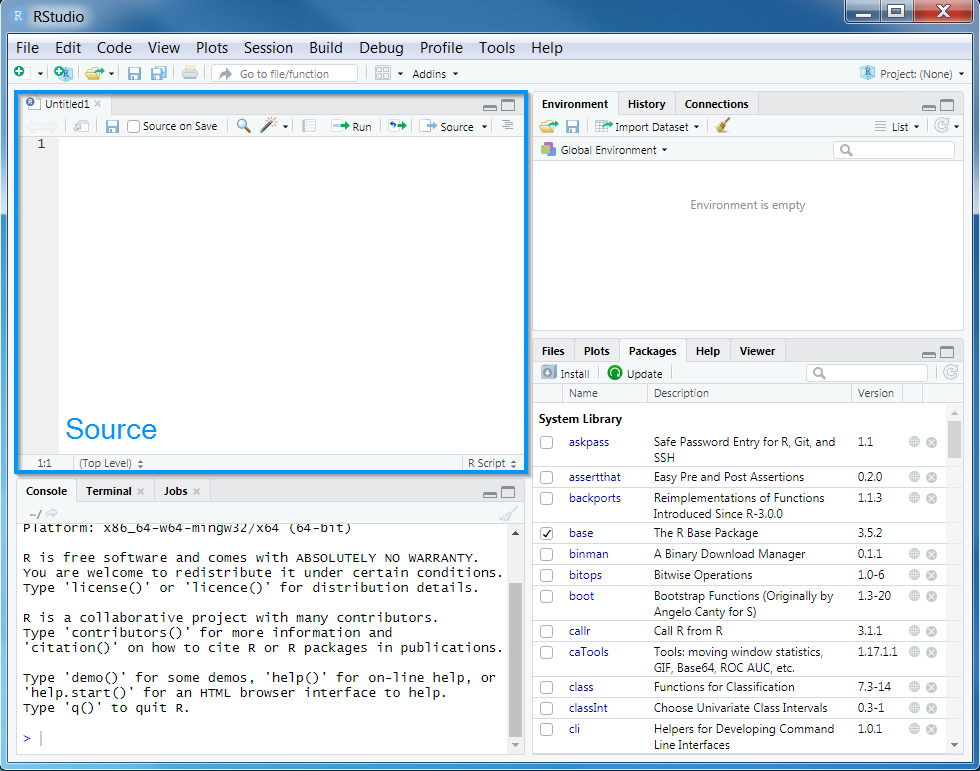
\includegraphics[width=0.7\linewidth]{images/rstudio-source} \end{center}

You can also make notes and write your answers to the workshop questions inside the R script. When writing notes and answers, add a \texttt{\#} symbol so that the text following the \texttt{\#} symbol is treated as a comment and not code. This means that you don't have to worry about highlighting specific parts of the script to avoid errors.

\begin{Shaded}
\begin{Highlighting}[]
\CommentTok{# this is a comment and R will ignore this text if you run it}
\CommentTok{# R will run the code below because it does not start with a # symbol}
\KeywordTok{print}\NormalTok{(}\StringTok{"this is not a comment"}\NormalTok{)}
\end{Highlighting}
\end{Shaded}

\begin{verbatim}
## [1] "this is not a comment"
\end{verbatim}

\begin{Shaded}
\begin{Highlighting}[]
\CommentTok{# you can also add comments to the same line of R code too}
\KeywordTok{print}\NormalTok{(}\StringTok{"this is also not a comment"}\NormalTok{) }\CommentTok{# but this is a comment}
\end{Highlighting}
\end{Shaded}

\begin{verbatim}
## [1] "this is also not a comment"
\end{verbatim}

\textbf{Remember to save your script regularly to ensure that you don't lose anything in the event that RStudio crashes (e.g.~using \texttt{Control\ +\ s} or \texttt{CMD\ +\ s})!}

\hypertarget{attaching-packages}{%
\section{Attaching packages}\label{attaching-packages}}

Now we will set up our R session for the workshop. Specifically, enter the following R code to attach the R packages used in this workshop.

\begin{Shaded}
\begin{Highlighting}[]
\CommentTok{# load packages}
\KeywordTok{library}\NormalTok{(tidyverse)}
\end{Highlighting}
\end{Shaded}

\begin{verbatim}
## Warning in system("timedatectl", intern = TRUE): running command 'timedatectl'
## had status 1
\end{verbatim}

\begin{Shaded}
\begin{Highlighting}[]
\KeywordTok{library}\NormalTok{(prioritizr)}
\KeywordTok{library}\NormalTok{(rgdal)}
\KeywordTok{library}\NormalTok{(raster)}
\KeywordTok{library}\NormalTok{(rgeos)}
\KeywordTok{library}\NormalTok{(mapview)}
\KeywordTok{library}\NormalTok{(units)}
\KeywordTok{library}\NormalTok{(scales)}
\KeywordTok{library}\NormalTok{(assertthat)}
\KeywordTok{library}\NormalTok{(gridExtra)}
\end{Highlighting}
\end{Shaded}

You should have already downloaded the data for the prioritizr module of this workshop. If you have not already done so, you can download it from here: \url{https://github.com/prioritizr/cibio-workshop/raw/master/data.zip}. After downloading the data, you can unzip the data into a new folder. Next, you will need to set the working directory to this new folder. To achieve this, click on the \emph{Session} button on the RStudio menu bar, then click \emph{Set Working Directory}, and then \emph{Choose Directory}.

\begin{center}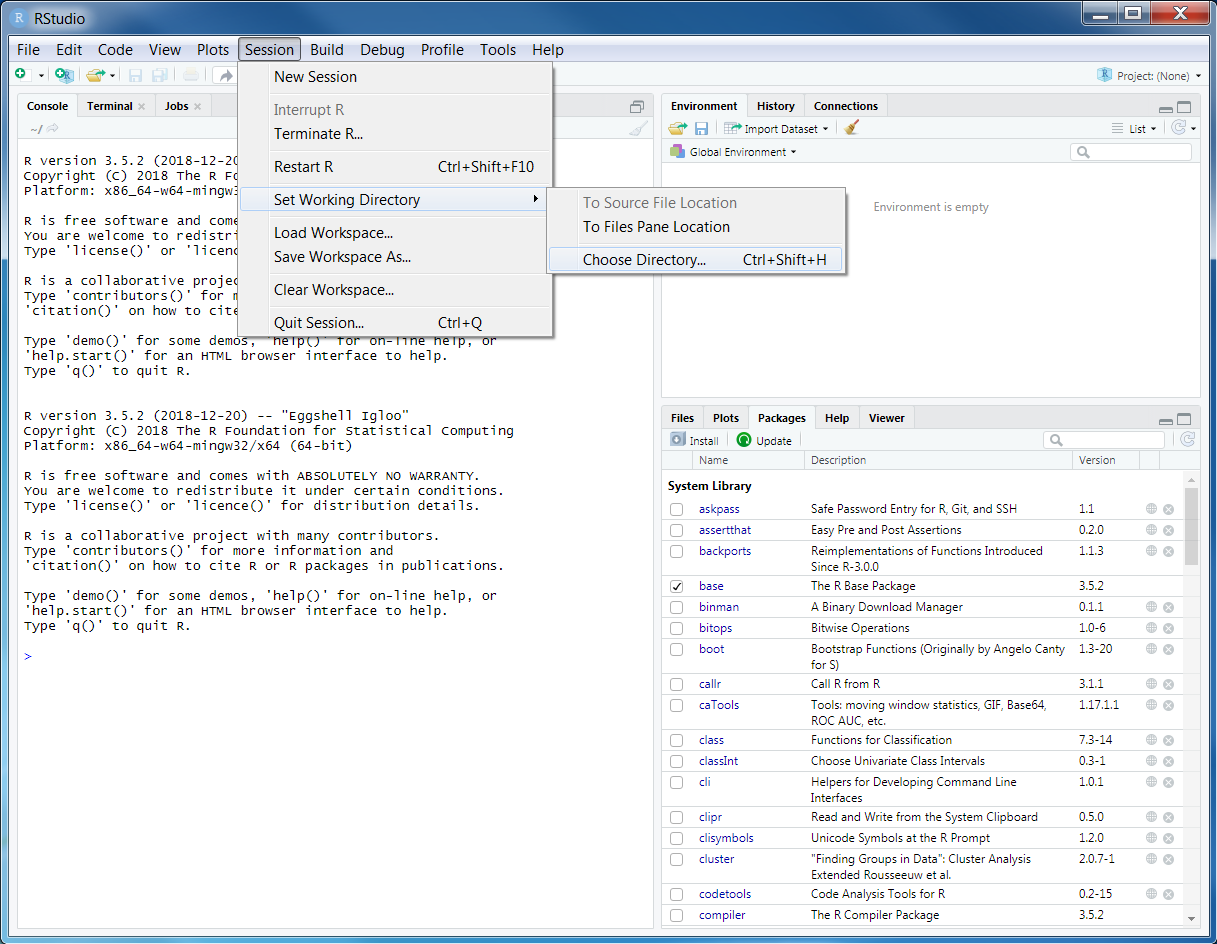
\includegraphics[width=0.7\linewidth]{images/rstudio-wd} \end{center}

\clearpage

Now navigate to the folder where you unzipped the data and select \emph{Open}. You can verify that you have correctly set the working directory using the following R code. You should see the output \texttt{TRUE} in the \emph{Console} panel.

\begin{Shaded}
\begin{Highlighting}[]
\KeywordTok{file.exists}\NormalTok{(}\StringTok{"data/pu.shp"}\NormalTok{)}
\end{Highlighting}
\end{Shaded}

\begin{verbatim}
## [1] TRUE
\end{verbatim}

\hypertarget{data-import}{%
\section{Data import}\label{data-import}}

Now that we have downloaded the dataset, we will need to import it into our R session. Specifically, this data was obtained from the ``Introduction to Marxan'' course and was originally a subset of a larger spatial prioritization project performed under contract to Australia's Department of Environment and Water Resources. It contains vector-based planning unit data (\texttt{pu.shp}) and the raster-based data describing the spatial distributions of 62 vegetation classes (\texttt{vegetation.tif}) in Tasmania, Australia. Please note this dataset is only provided for teaching purposes and should not be used for any real-world conservation planning. We can import the data into our R session using the following code.

\begin{Shaded}
\begin{Highlighting}[]
\CommentTok{# import planning unit data}
\NormalTok{pu_data <-}\StringTok{ }\KeywordTok{readOGR}\NormalTok{(}\StringTok{"data/pu.shp"}\NormalTok{)}
\end{Highlighting}
\end{Shaded}

\begin{verbatim}
## Warning: OGR support is provided by the sf and terra packages among others
\end{verbatim}

\begin{verbatim}
## Warning: OGR support is provided by the sf and terra packages among others
\end{verbatim}

\begin{verbatim}
## Warning: OGR support is provided by the sf and terra packages among others
\end{verbatim}

\begin{verbatim}
## Warning: OGR support is provided by the sf and terra packages among others
\end{verbatim}

\begin{verbatim}
## Warning: OGR support is provided by the sf and terra packages among others
\end{verbatim}

\begin{verbatim}
## Warning: OGR support is provided by the sf and terra packages among others
\end{verbatim}

\begin{verbatim}
## Warning: OGR support is provided by the sf and terra packages among others
\end{verbatim}

\begin{verbatim}
## OGR data source with driver: ESRI Shapefile 
## Source: "/mnt/d/Work/NCC/Training/prioritizr_workshop/NCC-workshop/data/pu.shp", layer: "pu"
## with 516 features
## It has 5 fields
\end{verbatim}

\begin{Shaded}
\begin{Highlighting}[]
\CommentTok{# format columns in planning unit data}
\NormalTok{pu_data}\OperatorTok{$}\NormalTok{locked_in <-}\StringTok{ }\KeywordTok{as.logical}\NormalTok{(pu_data}\OperatorTok{$}\NormalTok{locked_in)}
\NormalTok{pu_data}\OperatorTok{$}\NormalTok{locked_out <-}\StringTok{ }\KeywordTok{as.logical}\NormalTok{(pu_data}\OperatorTok{$}\NormalTok{locked_out)}

\CommentTok{# import vegetation data}
\NormalTok{veg_data <-}\StringTok{ }\KeywordTok{stack}\NormalTok{(}\StringTok{"data/vegetation.tif"}\NormalTok{)}
\end{Highlighting}
\end{Shaded}

\clearpage

\hypertarget{planning-unit-data}{%
\section{Planning unit data}\label{planning-unit-data}}

The planning unit data contains spatial data describing the geometry for each planning unit and attribute data with information about each planning unit (e.g.~cost values). Let's investigate the \texttt{pu\_data} object. The attribute data contains 5 columns with contain the following information:

\begin{itemize}
\tightlist
\item
  \texttt{id}: unique identifiers for each planning unit
\item
  \texttt{cost}: acquisition cost values for each planning unit (millions of Australian dollars).
\item
  \texttt{status}: status information for each planning unit (only relevant with Marxan)
\item
  \texttt{locked\_in}: logical values (i.e.~\texttt{TRUE}/\texttt{FALSE}) indicating if planning units are covered by protected areas or not.
\item
  \texttt{locked\_out}: logical values (i.e.~\texttt{TRUE}/\texttt{FALSE}) indicating if planning units cannot be managed as a protected area because they contain are too degraded.
\end{itemize}

\begin{Shaded}
\begin{Highlighting}[]
\CommentTok{# print a short summary of the data}
\KeywordTok{print}\NormalTok{(pu_data)}
\end{Highlighting}
\end{Shaded}

\begin{verbatim}
## class       : SpatialPolygonsDataFrame 
## features    : 516 
## extent      : 348703.2, 611932.4, 5167775, 5344516  (xmin, xmax, ymin, ymax)
## crs         : +proj=utm +zone=55 +south +datum=WGS84 +units=m +no_defs 
## variables   : 5
## names       :   id,             cost, status, locked_in, locked_out 
## min values  :  557, 3.59717531470679,      0,         0,          0 
## max values  : 1130,  47.238336402701,      2,         1,          1
\end{verbatim}

\begin{Shaded}
\begin{Highlighting}[]
\CommentTok{# plot the planning unit data}
\KeywordTok{plot}\NormalTok{(pu_data)}
\end{Highlighting}
\end{Shaded}

\begin{center}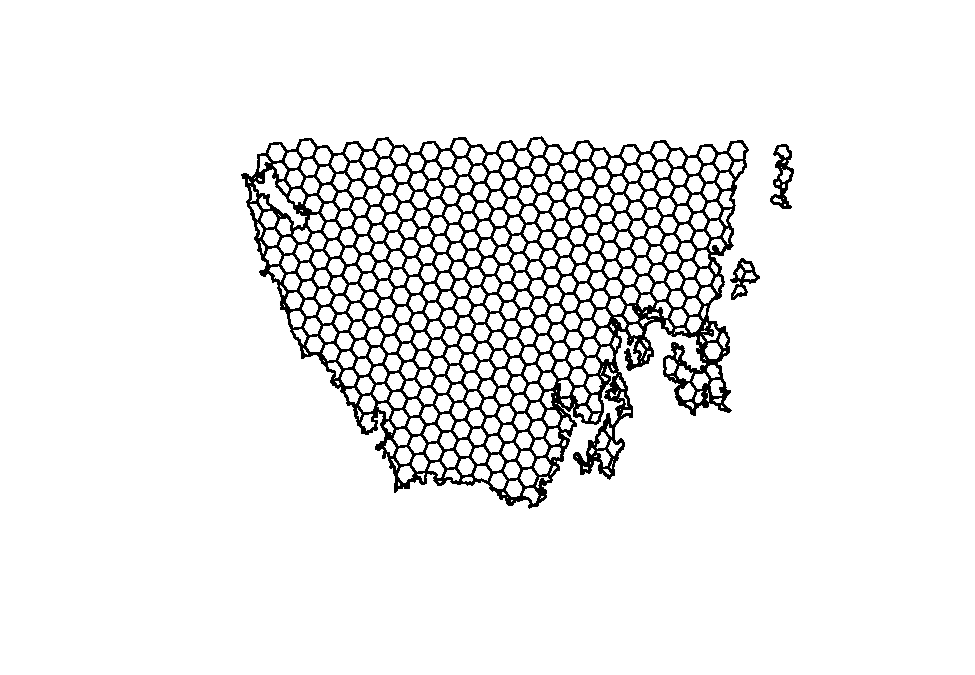
\includegraphics{prioritizr-workshop-manual_files/figure-latex/unnamed-chunk-15-1} \end{center}

\begin{Shaded}
\begin{Highlighting}[]
\CommentTok{# plot an interactive map of the planning unit data}
\KeywordTok{mapview}\NormalTok{(pu_data)}
\end{Highlighting}
\end{Shaded}

\begin{Shaded}
\begin{Highlighting}[]
\CommentTok{# print the structure of object}
\KeywordTok{str}\NormalTok{(pu_data, }\DataTypeTok{max.level =} \DecValTok{2}\NormalTok{)}
\end{Highlighting}
\end{Shaded}

\begin{verbatim}
## Formal class 'SpatialPolygonsDataFrame' [package "sp"] with 5 slots
##   ..@ data       :'data.frame':  516 obs. of  5 variables:
##   ..@ polygons   :List of 516
##   ..@ plotOrder  : int [1:516] 69 104 1 122 157 190 4 221 17 140 ...
##   ..@ bbox       : num [1:2, 1:2] 348703 5167775 611932 5344516
##   .. ..- attr(*, "dimnames")=List of 2
##   ..@ proj4string:Formal class 'CRS' [package "sp"] with 1 slot
##   ..$ comment: chr "TRUE"
\end{verbatim}

\begin{Shaded}
\begin{Highlighting}[]
\CommentTok{# print the class of the object}
\KeywordTok{class}\NormalTok{(pu_data)}
\end{Highlighting}
\end{Shaded}

\begin{verbatim}
## [1] "SpatialPolygonsDataFrame"
## attr(,"package")
## [1] "sp"
\end{verbatim}

\begin{Shaded}
\begin{Highlighting}[]
\CommentTok{# print the slots of the object}
\KeywordTok{slotNames}\NormalTok{(pu_data)}
\end{Highlighting}
\end{Shaded}

\begin{verbatim}
## [1] "data"        "polygons"    "plotOrder"   "bbox"        "proj4string"
\end{verbatim}

\begin{Shaded}
\begin{Highlighting}[]
\CommentTok{# print the geometry for the 80th planning unit}
\NormalTok{pu_data}\OperatorTok{@}\NormalTok{polygons[[}\DecValTok{80}\NormalTok{]]}
\end{Highlighting}
\end{Shaded}

\begin{verbatim}
## An object of class "Polygons"
## Slot "Polygons":
## [[1]]
## An object of class "Polygon"
## Slot "labpt":
## [1]  520772.4 5325744.8
## 
## Slot "area":
## [1] 64900653
## 
## Slot "hole":
## [1] FALSE
## 
## Slot "ringDir":
## [1] 1
## 
## Slot "coords":
##          [,1]    [,2]
## [1,] 518845.5 5321029
## [2,] 515940.4 5325147
## [3,] 517867.0 5329863
## [4,] 522700.2 5330460
## [5,] 525604.7 5326342
## [6,] 523676.6 5321627
## [7,] 518845.5 5321029
## 
## 
## 
## Slot "plotOrder":
## [1] 1
## 
## Slot "labpt":
## [1]  520772.4 5325744.8
## 
## Slot "ID":
## [1] "79"
## 
## Slot "area":
## [1] 64900653
\end{verbatim}

\begin{Shaded}
\begin{Highlighting}[]
\CommentTok{# print the coordinate reference system}
\KeywordTok{print}\NormalTok{(pu_data}\OperatorTok{@}\NormalTok{proj4string)}
\end{Highlighting}
\end{Shaded}

\begin{verbatim}
## Coordinate Reference System:
## Deprecated Proj.4 representation:
##  +proj=utm +zone=55 +south +datum=WGS84 +units=m +no_defs 
## WKT2 2019 representation:
## PROJCRS["WGS 84 / UTM zone 55S",
##     BASEGEOGCRS["WGS 84",
##         DATUM["World Geodetic System 1984",
##             ELLIPSOID["WGS 84",6378137,298.257223563,
##                 LENGTHUNIT["metre",1]]],
##         PRIMEM["Greenwich",0,
##             ANGLEUNIT["degree",0.0174532925199433]],
##         ID["EPSG",4326]],
##     CONVERSION["UTM zone 55S",
##         METHOD["Transverse Mercator",
##             ID["EPSG",9807]],
##         PARAMETER["Latitude of natural origin",0,
##             ANGLEUNIT["Degree",0.0174532925199433],
##             ID["EPSG",8801]],
##         PARAMETER["Longitude of natural origin",147,
##             ANGLEUNIT["Degree",0.0174532925199433],
##             ID["EPSG",8802]],
##         PARAMETER["Scale factor at natural origin",0.9996,
##             SCALEUNIT["unity",1],
##             ID["EPSG",8805]],
##         PARAMETER["False easting",500000,
##             LENGTHUNIT["metre",1],
##             ID["EPSG",8806]],
##         PARAMETER["False northing",10000000,
##             LENGTHUNIT["metre",1],
##             ID["EPSG",8807]]],
##     CS[Cartesian,2],
##         AXIS["(E)",east,
##             ORDER[1],
##             LENGTHUNIT["metre",1]],
##         AXIS["(N)",north,
##             ORDER[2],
##             LENGTHUNIT["metre",1]],
##     ID["EPSG",32755]]
\end{verbatim}

\begin{Shaded}
\begin{Highlighting}[]
\CommentTok{# print number of planning units (geometries) in the data}
\KeywordTok{nrow}\NormalTok{(pu_data)}
\end{Highlighting}
\end{Shaded}

\begin{verbatim}
## [1] 516
\end{verbatim}

\begin{Shaded}
\begin{Highlighting}[]
\CommentTok{# print the first six rows in the attribute data}
\KeywordTok{head}\NormalTok{(pu_data}\OperatorTok{@}\NormalTok{data)}
\end{Highlighting}
\end{Shaded}

\begin{verbatim}
##    id     cost status locked_in locked_out
## 0 557 29.74225      0     FALSE      FALSE
## 1 558 29.87703      0     FALSE      FALSE
## 2 574 28.60687      0     FALSE      FALSE
## 3 575 30.83416      0     FALSE      FALSE
## 4 576 38.75511      0     FALSE      FALSE
## 5 577 38.11618      2      TRUE      FALSE
\end{verbatim}

\begin{Shaded}
\begin{Highlighting}[]
\CommentTok{# print the first six values in the cost column of the attribute data}
\KeywordTok{head}\NormalTok{(pu_data}\OperatorTok{$}\NormalTok{cost)}
\end{Highlighting}
\end{Shaded}

\begin{verbatim}
## [1] 29.74225 29.87703 28.60687 30.83416 38.75511 38.11618
\end{verbatim}

\begin{Shaded}
\begin{Highlighting}[]
\CommentTok{# print the highest cost value}
\KeywordTok{max}\NormalTok{(pu_data}\OperatorTok{$}\NormalTok{cost)}
\end{Highlighting}
\end{Shaded}

\begin{verbatim}
## [1] 47.23834
\end{verbatim}

\begin{Shaded}
\begin{Highlighting}[]
\CommentTok{# print the smallest cost value}
\KeywordTok{min}\NormalTok{(pu_data}\OperatorTok{$}\NormalTok{cost)}
\end{Highlighting}
\end{Shaded}

\begin{verbatim}
## [1] 3.597175
\end{verbatim}

\begin{Shaded}
\begin{Highlighting}[]
\CommentTok{# print average cost value}
\KeywordTok{mean}\NormalTok{(pu_data}\OperatorTok{$}\NormalTok{cost)}
\end{Highlighting}
\end{Shaded}

\begin{verbatim}
## [1] 26.87393
\end{verbatim}

\begin{Shaded}
\begin{Highlighting}[]
\CommentTok{# plot a map of the planning unit cost data}
\KeywordTok{spplot}\NormalTok{(pu_data, }\StringTok{"cost"}\NormalTok{)}
\end{Highlighting}
\end{Shaded}

\begin{center}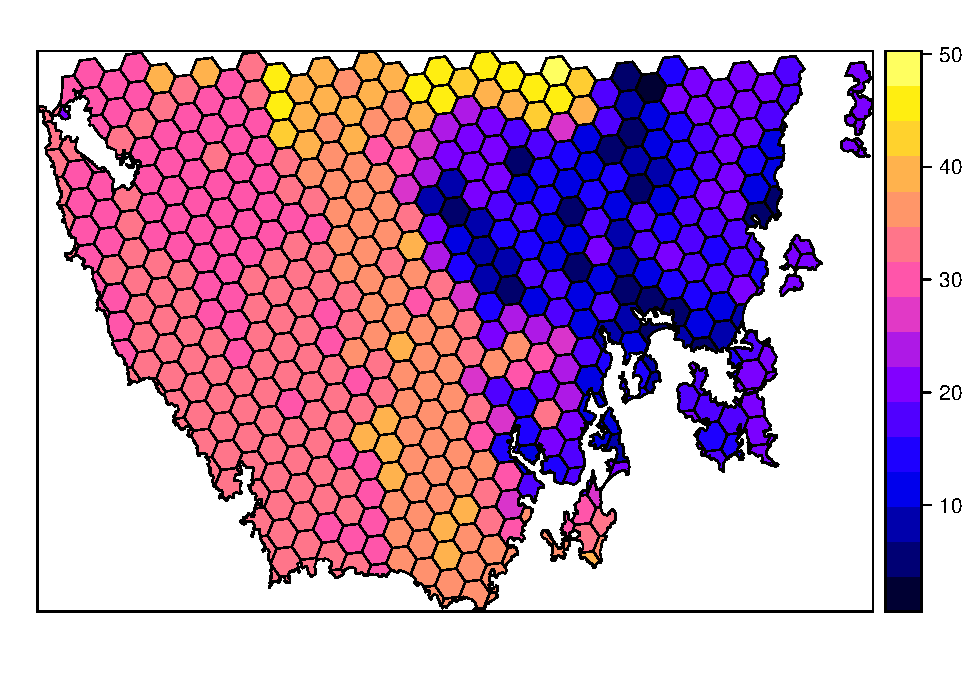
\includegraphics[width=0.6\linewidth]{prioritizr-workshop-manual_files/figure-latex/unnamed-chunk-17-1} \end{center}

\begin{Shaded}
\begin{Highlighting}[]
\CommentTok{# plot an interactive map of the planning unit cost data}
\KeywordTok{mapview}\NormalTok{(pu_data, }\DataTypeTok{zcol =} \StringTok{"cost"}\NormalTok{)}
\end{Highlighting}
\end{Shaded}

Now, you can try and answer some questions about the planning unit data.

\begin{rmdquestion}
\begin{enumerate}
\def\labelenumi{\arabic{enumi}.}
\tightlist
\item
  How many planning units are in the planning unit data?
\item
  What is the highest cost value?
\item
  How many planning units are covered by the protected areas (hint: \texttt{sum(x)})?
\item
  What is the proportion of the planning units that are covered by the protected areas (hint: \texttt{mean(x)})?
\item
  How many planning units are highly degraded (hint: \texttt{sum(x)})?
\item
  What is the proportion of planning units are highly degraded (hint: \texttt{mean(x)})?
\item
  Can you verify that all values in the \texttt{locked\_in} and \texttt{locked\_out} columns are zero or one (hint: \texttt{min(x)} and \texttt{max(x)})?.
\item
  Can you verify that none of the planning units are missing cost values (hint: \texttt{all(is.finite(x))})?.
\item
  Can you very that none of the planning units have duplicated identifiers? (hint: \texttt{sum(duplicated(x))})?
\item
  Is there a spatial pattern in the planning unit cost values (hint: use \texttt{spplot} to make a map).
\item
  Is there a spatial pattern in where most planning units are covered by protected areas (hint: use \texttt{spplot} to make a map).
\end{enumerate}
\end{rmdquestion}

\clearpage

\hypertarget{vegetation-data}{%
\section{Vegetation data}\label{vegetation-data}}

The vegetation data describes the spatial distribution of 62 vegetation classes in the study area. This data is in a raster format and so the data are organized using a square grid comprising square grid cells that are each the same size. In our case, the raster data contains multiple layers (also called ``bands'') and each layer has corresponds to a spatial grid with exactly the same area and has exactly the same dimensionality (i.e.~number of rows, columns, and cells). In this dataset, there are 62 different regular spatial grids layered on top of each other -- with each layer corresponding to a different vegetation class -- and each of these layers contains a grid with 164 rows, 326 columns, and 53464 cells. Within each layer, each cell corresponds to a 0.967 by 1.02 km square. The values associated with each grid cell indicate the (one) presence or (zero) absence of a given vegetation class in the cell.

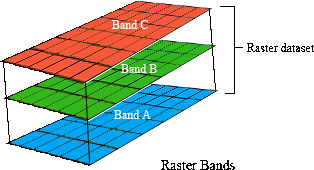
\includegraphics{images/rasterbands.png}

Let's explore the vegetation data.

\begin{Shaded}
\begin{Highlighting}[]
\CommentTok{# print a short summary of the data}
\KeywordTok{print}\NormalTok{(veg_data)}
\end{Highlighting}
\end{Shaded}

\begin{verbatim}
## class      : RasterStack 
## dimensions : 164, 326, 53464, 32  (nrow, ncol, ncell, nlayers)
## resolution : 967, 1020  (x, y)
## extent     : 298636.7, 613878.7, 5167756, 5335036  (xmin, xmax, ymin, ymax)
## crs        : +proj=utm +zone=55 +south +datum=WGS84 +units=m +no_defs 
## names      : vegetation_1, vegetation_2, vegetation_3, vegetation_4, vegetation_5, vegetation_6, vegetation_7, vegetation_8, vegetation_9, vegetation_10, vegetation_11, vegetation_12, vegetation_13, vegetation_14, vegetation_15, ... 
## min values :            0,            0,            0,            0,            0,            0,            0,            0,            0,             0,             0,             0,             0,             0,             0, ... 
## max values :            1,            1,            1,            1,            1,            1,            1,            1,            1,             1,             1,             1,             1,             1,             1, ...
\end{verbatim}

\begin{Shaded}
\begin{Highlighting}[]
\CommentTok{# plot a map of the 36th vegetation class}
\KeywordTok{plot}\NormalTok{(veg_data[[}\DecValTok{32}\NormalTok{]])}
\end{Highlighting}
\end{Shaded}

\begin{center}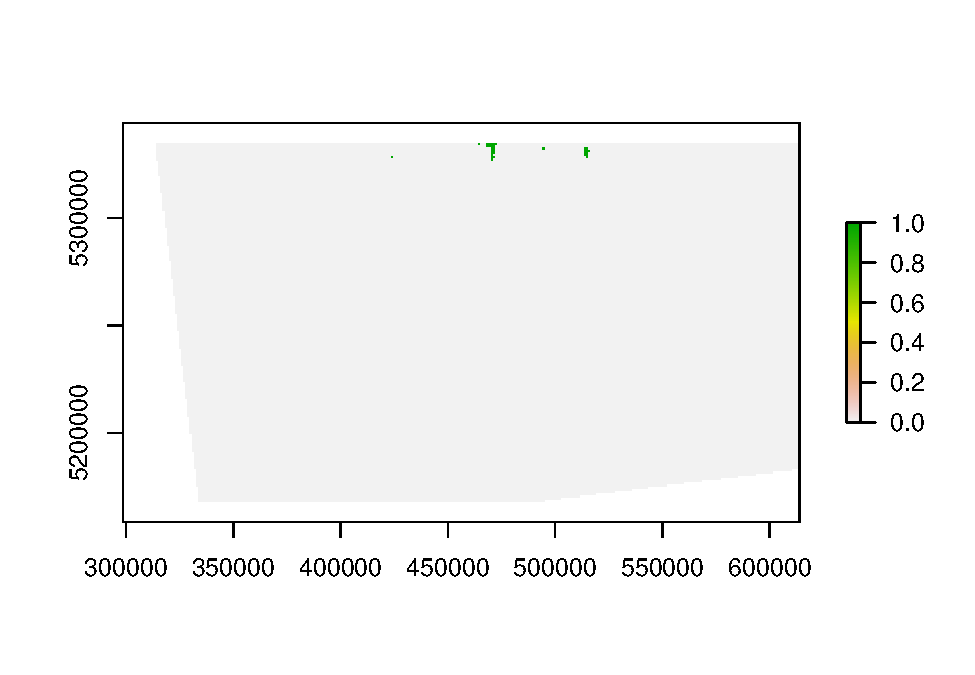
\includegraphics{prioritizr-workshop-manual_files/figure-latex/unnamed-chunk-20-1} \end{center}

\begin{Shaded}
\begin{Highlighting}[]
\CommentTok{# plot an interactive map of the 36th vegetation class}
\KeywordTok{mapview}\NormalTok{(veg_data[[}\DecValTok{32}\NormalTok{]])}
\end{Highlighting}
\end{Shaded}

\begin{Shaded}
\begin{Highlighting}[]
\CommentTok{# print number of rows in the data}
\KeywordTok{nrow}\NormalTok{(veg_data)}
\end{Highlighting}
\end{Shaded}

\begin{verbatim}
## [1] 164
\end{verbatim}

\begin{Shaded}
\begin{Highlighting}[]
\CommentTok{# print number of columns  in the data}
\KeywordTok{ncol}\NormalTok{(veg_data)}
\end{Highlighting}
\end{Shaded}

\begin{verbatim}
## [1] 326
\end{verbatim}

\begin{Shaded}
\begin{Highlighting}[]
\CommentTok{# print number of cells in the data}
\KeywordTok{ncell}\NormalTok{(veg_data)}
\end{Highlighting}
\end{Shaded}

\begin{verbatim}
## [1] 53464
\end{verbatim}

\begin{Shaded}
\begin{Highlighting}[]
\CommentTok{# print number of layers in the data}
\KeywordTok{nlayers}\NormalTok{(veg_data)}
\end{Highlighting}
\end{Shaded}

\begin{verbatim}
## [1] 32
\end{verbatim}

\begin{Shaded}
\begin{Highlighting}[]
\CommentTok{# print  resolution on the x-axis}
\KeywordTok{xres}\NormalTok{(veg_data)}
\end{Highlighting}
\end{Shaded}

\begin{verbatim}
## [1] 967
\end{verbatim}

\begin{Shaded}
\begin{Highlighting}[]
\CommentTok{# print resolution on the y-axis}
\KeywordTok{yres}\NormalTok{(veg_data)}
\end{Highlighting}
\end{Shaded}

\begin{verbatim}
## [1] 1020
\end{verbatim}

\begin{Shaded}
\begin{Highlighting}[]
\CommentTok{# print spatial extent of the grid, i.e. coordinates for corners}
\KeywordTok{extent}\NormalTok{(veg_data)}
\end{Highlighting}
\end{Shaded}

\begin{verbatim}
## class      : Extent 
## xmin       : 298636.7 
## xmax       : 613878.7 
## ymin       : 5167756 
## ymax       : 5335036
\end{verbatim}

\begin{Shaded}
\begin{Highlighting}[]
\CommentTok{# print the coordinate reference system}
\KeywordTok{print}\NormalTok{(veg_data}\OperatorTok{@}\NormalTok{crs)}
\end{Highlighting}
\end{Shaded}

\begin{verbatim}
## Coordinate Reference System:
## Deprecated Proj.4 representation:
##  +proj=utm +zone=55 +south +datum=WGS84 +units=m +no_defs 
## WKT2 2019 representation:
## PROJCRS["unknown",
##     BASEGEOGCRS["unknown",
##         DATUM["World Geodetic System 1984",
##             ELLIPSOID["WGS 84",6378137,298.257223563,
##                 LENGTHUNIT["metre",1]],
##             ID["EPSG",6326]],
##         PRIMEM["Greenwich",0,
##             ANGLEUNIT["degree",0.0174532925199433],
##             ID["EPSG",8901]]],
##     CONVERSION["UTM zone 55S",
##         METHOD["Transverse Mercator",
##             ID["EPSG",9807]],
##         PARAMETER["Latitude of natural origin",0,
##             ANGLEUNIT["degree",0.0174532925199433],
##             ID["EPSG",8801]],
##         PARAMETER["Longitude of natural origin",147,
##             ANGLEUNIT["degree",0.0174532925199433],
##             ID["EPSG",8802]],
##         PARAMETER["Scale factor at natural origin",0.9996,
##             SCALEUNIT["unity",1],
##             ID["EPSG",8805]],
##         PARAMETER["False easting",500000,
##             LENGTHUNIT["metre",1],
##             ID["EPSG",8806]],
##         PARAMETER["False northing",10000000,
##             LENGTHUNIT["metre",1],
##             ID["EPSG",8807]],
##         ID["EPSG",17055]],
##     CS[Cartesian,2],
##         AXIS["(E)",east,
##             ORDER[1],
##             LENGTHUNIT["metre",1,
##                 ID["EPSG",9001]]],
##         AXIS["(N)",north,
##             ORDER[2],
##             LENGTHUNIT["metre",1,
##                 ID["EPSG",9001]]]]
\end{verbatim}

\begin{Shaded}
\begin{Highlighting}[]
\CommentTok{# print a summary of the first layer in the stack}
\KeywordTok{print}\NormalTok{(veg_data[[}\DecValTok{1}\NormalTok{]])}
\end{Highlighting}
\end{Shaded}

\begin{verbatim}
## class      : RasterLayer 
## band       : 1  (of  32  bands)
## dimensions : 164, 326, 53464  (nrow, ncol, ncell)
## resolution : 967, 1020  (x, y)
## extent     : 298636.7, 613878.7, 5167756, 5335036  (xmin, xmax, ymin, ymax)
## crs        : +proj=utm +zone=55 +south +datum=WGS84 +units=m +no_defs 
## source     : vegetation.tif 
## names      : vegetation_1 
## values     : 0, 1  (min, max)
\end{verbatim}

\begin{Shaded}
\begin{Highlighting}[]
\CommentTok{# print the value in the 800th cell in the first layer of the stack}
\KeywordTok{print}\NormalTok{(veg_data[[}\DecValTok{1}\NormalTok{]][}\DecValTok{800}\NormalTok{])}
\end{Highlighting}
\end{Shaded}

\begin{verbatim}
##   
## 0
\end{verbatim}

\begin{Shaded}
\begin{Highlighting}[]
\CommentTok{# print the value of the cell located in the 30th row and the 60th column of}
\CommentTok{# the first layer}
\KeywordTok{print}\NormalTok{(veg_data[[}\DecValTok{1}\NormalTok{]][}\DecValTok{30}\NormalTok{, }\DecValTok{60}\NormalTok{])}
\end{Highlighting}
\end{Shaded}

\begin{verbatim}
##   
## 0
\end{verbatim}

\begin{Shaded}
\begin{Highlighting}[]
\CommentTok{# calculate the sum of all the cell values in the first layer}
\KeywordTok{cellStats}\NormalTok{(veg_data[[}\DecValTok{1}\NormalTok{]], }\StringTok{"sum"}\NormalTok{)}
\end{Highlighting}
\end{Shaded}

\begin{verbatim}
## [1] 17
\end{verbatim}

\begin{Shaded}
\begin{Highlighting}[]
\CommentTok{# calculate the maximum value of all the cell values in the first layer}
\KeywordTok{cellStats}\NormalTok{(veg_data[[}\DecValTok{1}\NormalTok{]], }\StringTok{"max"}\NormalTok{)}
\end{Highlighting}
\end{Shaded}

\begin{verbatim}
## [1] 1
\end{verbatim}

\begin{Shaded}
\begin{Highlighting}[]
\CommentTok{# calculate the minimum value of all the cell values in the first layer}
\KeywordTok{cellStats}\NormalTok{(veg_data[[}\DecValTok{1}\NormalTok{]], }\StringTok{"min"}\NormalTok{)}
\end{Highlighting}
\end{Shaded}

\begin{verbatim}
## [1] 0
\end{verbatim}

\begin{Shaded}
\begin{Highlighting}[]
\CommentTok{# calculate the mean value of all the cell values in the first layer}
\KeywordTok{cellStats}\NormalTok{(veg_data[[}\DecValTok{1}\NormalTok{]], }\StringTok{"mean"}\NormalTok{)}
\end{Highlighting}
\end{Shaded}

\begin{verbatim}
## [1] 0.00035239
\end{verbatim}

\clearpage

\begin{Shaded}
\begin{Highlighting}[]
\CommentTok{# calculate the maximum value in each layer}
\KeywordTok{as_tibble}\NormalTok{(}\KeywordTok{data.frame}\NormalTok{(}\DataTypeTok{max =} \KeywordTok{cellStats}\NormalTok{(veg_data, }\StringTok{"max"}\NormalTok{)))}
\end{Highlighting}
\end{Shaded}

\begin{verbatim}
## # A tibble: 32 x 1
##      max
##    <dbl>
##  1     1
##  2     1
##  3     1
##  4     1
##  5     1
##  6     1
##  7     1
##  8     1
##  9     1
## 10     1
## # i 22 more rows
\end{verbatim}

Now, you can try and answer some questions about the vegetation data.

\begin{rmdquestion}
\begin{enumerate}
\def\labelenumi{\arabic{enumi}.}
\tightlist
\item
  What part of the study area is the 51st vegetation class found in (hint: make a map)?
\item
  What proportion of cells contain the 12th vegetation class?
\item
  Which vegetation class is present in the greatest number of cells?
\item
  The planning unit data and the vegetation data should have the same coordinate reference system. Can you check if they are the same?
\end{enumerate}
\end{rmdquestion}

\hypertarget{gap-analysis}{%
\chapter{Gap analysis}\label{gap-analysis}}

\hypertarget{introduction-1}{%
\section{Introduction}\label{introduction-1}}

Before we begin to prioritize areas for protected area establishment, we should first understand how well existing protected areas are conserving our biodiversity features (i.e.~native vegetation classes in Tasmania, Australia). This step is critical: we cannot develop plans to improve conservation of biodiversity if we don't understand how well existing policies are currently conserving biodiversity! To achieve this, we can perform a ``gap analysis''. A gap analysis involves calculating how well each of our biodiversity features (i.e.~vegetation classes in this exercise) are represented (covered) by protected areas. Next, we compare current representation by protected areas of each feature (e.g.~5\% of their spatial distribution covered by protected areas) to a target threshold (e.g.~20\% of their spatial distribution covered by protected areas). This target threshold denotes the minimum amount (e.g.~minimum proportion of spatial distribution) that we need of each feature to be represented in the protected area system. Ideally, targets should be based on an estimate of how much area or habitat is needed for ecosystem function or species persistence. In practice, targets are generally set using simple rules of thumb (e.g.~10\% or 20\%), policy (17\%; \url{https://www.cbd.int/sp/targets/rationale/target-11}) or standard practices (e.g.~setting targets for species based on geographic range size) \citep{r1, r2}.

\hypertarget{feature-abundance}{%
\section{Feature abundance}\label{feature-abundance}}

Now we will perform some preliminary calculations to explore the data. First, we will calculate how much of each vegetation feature occurs inside each planning unit (i.e.~the abundance of the features). To achieve this, we will use the \texttt{problem} function to create an empty conservation planning problem that only contains the planning unit and biodiversity data. We will then use the \texttt{feature\_abundances} function to calculate the total amount of each feature in each planning unit.

\begin{Shaded}
\begin{Highlighting}[]
\CommentTok{# create prioritizr problem with only the data}
\NormalTok{p0 <-}\StringTok{ }\KeywordTok{problem}\NormalTok{(pu_data, veg_data, }\DataTypeTok{cost_column =} \StringTok{"cost"}\NormalTok{)}
\end{Highlighting}
\end{Shaded}

\begin{verbatim}
## Warning: Support for sp package will be deprecated.
## i Use `sf::st_as_sf()` to convert data for future compatibility.
\end{verbatim}

\begin{verbatim}
## Warning: Support for raster package will be deprecated.
## i Use `terra::rast()` to convert data for future compatibility.
\end{verbatim}

\begin{Shaded}
\begin{Highlighting}[]
\CommentTok{# print empty problem,}
\CommentTok{# we can see that only the cost and feature data are defined}
\KeywordTok{print}\NormalTok{(p0)}
\end{Highlighting}
\end{Shaded}

\begin{verbatim}
## A conservation problem (<ConservationProblem>)
\end{verbatim}

\begin{verbatim}
## +@data
\end{verbatim}

\begin{verbatim}
## |+@features:    "vegetation_1", "vegetation_2", "vegetation_3", "vegetation_4" , ... (32 total)
\end{verbatim}

\begin{verbatim}
## |\@planning units:
\end{verbatim}

\begin{verbatim}
## | +@data:       <SpatialPolygonsDataFrame> (516 total)
\end{verbatim}

\begin{verbatim}
## | +@costs:      continuous values (between 3.5972 and 47.2383)
\end{verbatim}

\begin{verbatim}
## | +@extent:     348703.1831, 5167774.5993, 611932.4474, 5344516.4109 (xmin, ymin, xmax, ymax)
\end{verbatim}

\begin{verbatim}
## | \@CRS:        WGS 84 / UTM zone 55S
\end{verbatim}

\begin{verbatim}
## +@formulation
\end{verbatim}

\begin{verbatim}
## |+@objective:   none specified
\end{verbatim}

\begin{verbatim}
## |+@penalties:   none specified
\end{verbatim}

\begin{verbatim}
## |+@targets:     none specified
\end{verbatim}

\begin{verbatim}
## |+@constraints: none specified
\end{verbatim}

\begin{verbatim}
## |\@decisions:   binary decision
\end{verbatim}

\begin{verbatim}
## \@optimization
\end{verbatim}

\begin{verbatim}
##  +@portfolio:   shuffle portfolio (`number_solutions` = 1, ...)
\end{verbatim}

\begin{verbatim}
##  \@solver:      gurobi solver (`gap` = 0.1, `time_limit` = 2147483647, `first_feasible` = FALSE, ...)
\end{verbatim}

\begin{verbatim}
## # i Use `summary(...)` to see complete formulation.
\end{verbatim}

\begin{Shaded}
\begin{Highlighting}[]
\CommentTok{# calculate amount of each feature in each planning unit}
\NormalTok{abundance_data <-}\StringTok{ }\KeywordTok{feature_abundances}\NormalTok{(p0)}

\CommentTok{# print abundance data}
\KeywordTok{print}\NormalTok{(abundance_data)}
\end{Highlighting}
\end{Shaded}

\begin{verbatim}
## # A tibble: 32 x 3
##    feature       absolute_abundance relative_abundance
##    <chr>                      <dbl>              <dbl>
##  1 vegetation_1                16.0                  1
##  2 vegetation_2                14.3                  1
##  3 vegetation_3                10.4                  1
##  4 vegetation_4                17.8                  1
##  5 vegetation_5                13.0                  1
##  6 vegetation_6                14.3                  1
##  7 vegetation_7                20.0                  1
##  8 vegetation_8                14.0                  1
##  9 vegetation_9                18.0                  1
## 10 vegetation_10               20.0                  1
## # i 22 more rows
\end{verbatim}

\clearpage

\begin{Shaded}
\begin{Highlighting}[]
\CommentTok{# note that only the first ten rows are printed,}
\CommentTok{# this is because the abundance_data object is a tibble (i.e. tbl_df) object}
\CommentTok{# and not a standard data.frame object}
\KeywordTok{print}\NormalTok{(}\KeywordTok{class}\NormalTok{(abundance_data))}
\end{Highlighting}
\end{Shaded}

\begin{verbatim}
## [1] "tbl_df"     "tbl"        "data.frame"
\end{verbatim}

\begin{Shaded}
\begin{Highlighting}[]
\CommentTok{# we can print all of the rows in abundance_data like this}
\KeywordTok{print}\NormalTok{(abundance_data, }\DataTypeTok{n =} \OtherTok{Inf}\NormalTok{)}
\end{Highlighting}
\end{Shaded}

\begin{verbatim}
## # A tibble: 32 x 3
##    feature       absolute_abundance relative_abundance
##    <chr>                      <dbl>              <dbl>
##  1 vegetation_1                16.0                  1
##  2 vegetation_2                14.3                  1
##  3 vegetation_3                10.4                  1
##  4 vegetation_4                17.8                  1
##  5 vegetation_5                13.0                  1
##  6 vegetation_6                14.3                  1
##  7 vegetation_7                20.0                  1
##  8 vegetation_8                14.0                  1
##  9 vegetation_9                18.0                  1
## 10 vegetation_10               20.0                  1
## 11 vegetation_11               23.6                  1
## 12 vegetation_12              748.                   1
## 13 vegetation_13              126.                   1
## 14 vegetation_14               10.5                  1
## 15 vegetation_15               17.5                  1
## 16 vegetation_16               15.0                  1
## 17 vegetation_17              213.                   1
## 18 vegetation_18               14.3                  1
## 19 vegetation_19               17.1                  1
## 20 vegetation_20               21.4                  1
## 21 vegetation_21               18.6                  1
## 22 vegetation_22              297.                   1
## 23 vegetation_23               20.3                  1
## 24 vegetation_24              165.                   1
## 25 vegetation_25              716.                   1
## 26 vegetation_26               24.0                  1
## 27 vegetation_27               18.8                  1
## 28 vegetation_28               17.5                  1
## 29 vegetation_29               24.7                  1
## 30 vegetation_30               59.0                  1
## 31 vegetation_31               60.0                  1
## 32 vegetation_32               32.0                  1
\end{verbatim}

The \texttt{abundance\_data} object contains three columns. The \texttt{feature} column contains the name of each feature (derived from \texttt{names(veg\_data})), the \texttt{absolute\_abundance} column contains the total amount of each feature in all the planning units, and the \texttt{relative\_abundance} column contains the total amount of each feature in the planning units expressed as a proportion of the total amount in the underlying raster data. Since all the raster cells containing vegetation overlap with the planning units, all of the values in the \texttt{relative\_abundance} column are equal to one (meaning 100\%)---except for the 61st feature which has a value on \texttt{NaN} because it does not occur in the study area at all (i.e.~all of its raster values are zeros). Now let's add a new column with the feature abundances expressed in area units (i.e.~km\textsuperscript{2}).

\begin{Shaded}
\begin{Highlighting}[]
\CommentTok{# add new column with feature abundances in km^2}
\NormalTok{abundance_data}\OperatorTok{$}\NormalTok{absolute_abundance_km2 <-}
\StringTok{  }\NormalTok{(abundance_data}\OperatorTok{$}\NormalTok{absolute_abundance }\OperatorTok{*}\StringTok{ }\KeywordTok{prod}\NormalTok{(}\KeywordTok{res}\NormalTok{(veg_data))) }\OperatorTok
\StringTok{  }\KeywordTok{set_units}\NormalTok{(m}\OperatorTok{^}\DecValTok{2}\NormalTok{) }\OperatorTok
\StringTok{  }\KeywordTok{set_units}\NormalTok{(km}\OperatorTok{^}\DecValTok{2}\NormalTok{)}

\CommentTok{# print abundance data}
\KeywordTok{print}\NormalTok{(abundance_data)}
\end{Highlighting}
\end{Shaded}

\begin{verbatim}
## # A tibble: 32 x 4
##    feature       absolute_abundance relative_abundance absolute_abundance_km2
##    <chr>                      <dbl>              <dbl>                 [km^2]
##  1 vegetation_1                16.0                  1                   15.8
##  2 vegetation_2                14.3                  1                   14.1
##  3 vegetation_3                10.4                  1                   10.2
##  4 vegetation_4                17.8                  1                   17.6
##  5 vegetation_5                13.0                  1                   12.8
##  6 vegetation_6                14.3                  1                   14.1
##  7 vegetation_7                20.0                  1                   19.7
##  8 vegetation_8                14.0                  1                   13.9
##  9 vegetation_9                18.0                  1                   17.8
## 10 vegetation_10               20.0                  1                   19.7
## # i 22 more rows
\end{verbatim}

Now let's explore the abundance data.

\begin{Shaded}
\begin{Highlighting}[]
\CommentTok{# calculate the average abundance of the features}
\KeywordTok{mean}\NormalTok{(abundance_data}\OperatorTok{$}\NormalTok{absolute_abundance_km2)}
\end{Highlighting}
\end{Shaded}

\begin{verbatim}
## 86.82948 [km^2]
\end{verbatim}

\begin{Shaded}
\begin{Highlighting}[]
\CommentTok{# plot histogram of the features' abundances}
\KeywordTok{hist}\NormalTok{(abundance_data}\OperatorTok{$}\NormalTok{absolute_abundance_km2, }\DataTypeTok{main =} \StringTok{"Feature abundances"}\NormalTok{)}
\end{Highlighting}
\end{Shaded}

\begin{center}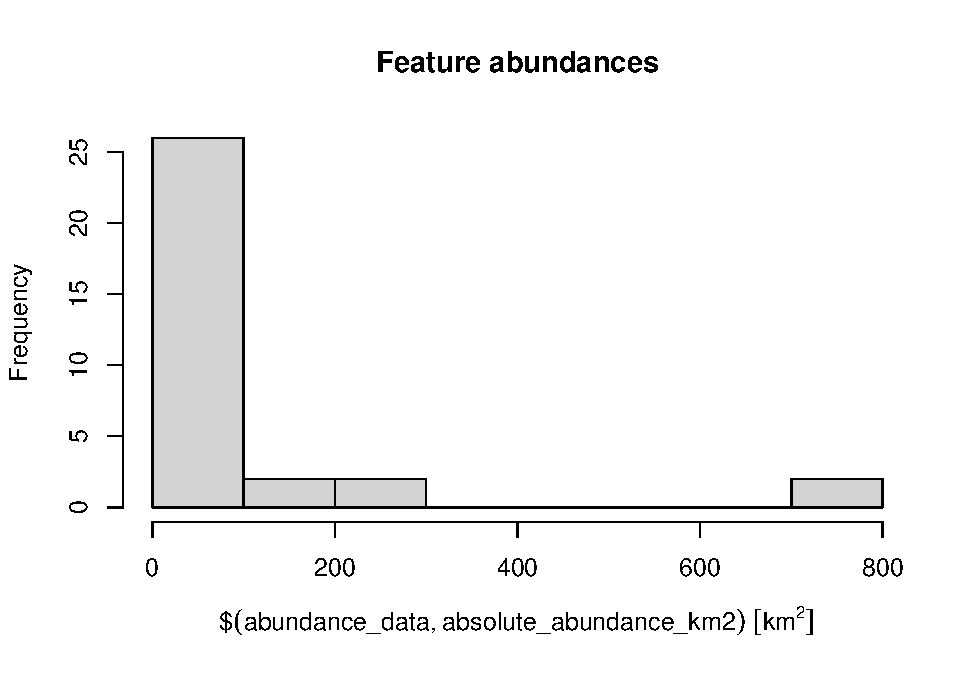
\includegraphics{prioritizr-workshop-manual_files/figure-latex/unnamed-chunk-29-1} \end{center}

\begin{Shaded}
\begin{Highlighting}[]
\CommentTok{# find the abundance of the feature with the largest abundance}
\KeywordTok{max}\NormalTok{(abundance_data}\OperatorTok{$}\NormalTok{absolute_abundance_km2)}
\end{Highlighting}
\end{Shaded}

\begin{verbatim}
## 737.982 [km^2]
\end{verbatim}

\begin{Shaded}
\begin{Highlighting}[]
\CommentTok{# find the name of the feature with the largest abundance}
\NormalTok{abundance_data}\OperatorTok{$}\NormalTok{feature[}\KeywordTok{which.max}\NormalTok{(abundance_data}\OperatorTok{$}\NormalTok{absolute_abundance_km2)]}
\end{Highlighting}
\end{Shaded}

\begin{verbatim}
## [1] "vegetation_12"
\end{verbatim}

Now, try to answer the following questions.

\begin{rmdquestion}
\begin{enumerate}
\def\labelenumi{\arabic{enumi}.}
\tightlist
\item
  What is the median abundance of the features (hint: \texttt{median})?
\item
  What is the abundance of the feature with smallest abundance?
\item
  What is the name of the feature with smallest abundance?
\item
  What is the total abundance of all features in the planning units summed together?
\item
  How many features have a total abundance greater than 100 km\^{}2 (hint: \texttt{sum(abundance\_values\ \textgreater{}\ set\_units(threshold\_value,\ km\^{}2)})?
\end{enumerate}
\end{rmdquestion}

\hypertarget{feature-representation-by-protected-areas}{%
\section{Feature representation by protected areas}\label{feature-representation-by-protected-areas}}

After calculating the total amount of each feature in the planning units (i.e.~the features' abundances), we will now calculate the amount of each feature in the planning units that are covered by protected areas (i.e.~feature representation by protected areas). We can complete this task using the \texttt{feature\_representation} function. This function requires (i) a conservation problem object with the planning unit and biodiversity data and also (ii) an object representing a solution to the problem (i.e an object in the same format as the planning unit data with values indicating if the planning units are selected or not).

\begin{Shaded}
\begin{Highlighting}[]
\CommentTok{# create column in planning unit data with binary values (zeros and ones)}
\CommentTok{# indicating if a planning unit is covered by protected areas or not}
\NormalTok{pu_data}\OperatorTok{$}\NormalTok{pa_status <-}\StringTok{ }\KeywordTok{as.numeric}\NormalTok{(pu_data}\OperatorTok{$}\NormalTok{locked_in)}

\CommentTok{# calculate feature representation by protected areas}
\NormalTok{repr_data <-}\StringTok{ }\KeywordTok{eval_feature_representation_summary}\NormalTok{(p0, pu_data[, }\StringTok{"pa_status"}\NormalTok{])}
\end{Highlighting}
\end{Shaded}

\begin{verbatim}
## Warning: Support for sp package will be deprecated.
## i Use `sf::st_as_sf()` to convert data for future compatibility.
\end{verbatim}

\begin{Shaded}
\begin{Highlighting}[]
\CommentTok{# print feature representation data}
\KeywordTok{print}\NormalTok{(repr_data)}
\end{Highlighting}
\end{Shaded}

\begin{verbatim}
## # A tibble: 32 x 5
##    summary feature       total_amount absolute_held relative_held
##    <chr>   <chr>                <dbl>         <dbl>         <dbl>
##  1 overall vegetation_1          16.0         0            0     
##  2 overall vegetation_2          14.3         0            0     
##  3 overall vegetation_3          10.4         0            0     
##  4 overall vegetation_4          17.8         0            0     
##  5 overall vegetation_5          13.0         0            0     
##  6 overall vegetation_6          14.3         0            0     
##  7 overall vegetation_7          20.0         0            0     
##  8 overall vegetation_8          14.0         0            0     
##  9 overall vegetation_9          18.0         0.846        0.0470
## 10 overall vegetation_10         20.0         0            0     
## # i 22 more rows
\end{verbatim}

Similar to the abundance data before, the \texttt{repr\_data} object contains three columns. The \texttt{feature} column contains the name of each feature, the \texttt{absolute\_held} column shows the total amount of each feature held in the solution (i.e.~the planning units covered by protected areas), and the \texttt{relative\_held} column shows the proportion of each feature held in the solution (i.e.~the proportion of each feature's spatial distribution held in protected areas). Since the \texttt{absolute\_held} values correspond to the number of grid cells in the \texttt{veg\_data} object with overlap with protected areas, let's convert them to area units (i.e.~km\textsuperscript{2}) so we can report them.

\begin{Shaded}
\begin{Highlighting}[]
\CommentTok{# add new column with the areas represented in km^2}
\NormalTok{repr_data}\OperatorTok{$}\NormalTok{absolute_held_km2 <-}
\StringTok{  }\NormalTok{(repr_data}\OperatorTok{$}\NormalTok{absolute_held }\OperatorTok{*}\StringTok{ }\KeywordTok{prod}\NormalTok{(}\KeywordTok{res}\NormalTok{(veg_data))) }\OperatorTok
\StringTok{  }\KeywordTok{set_units}\NormalTok{(m}\OperatorTok{^}\DecValTok{2}\NormalTok{) }\OperatorTok
\StringTok{  }\KeywordTok{set_units}\NormalTok{(km}\OperatorTok{^}\DecValTok{2}\NormalTok{)}

\CommentTok{# print representation data}
\KeywordTok{print}\NormalTok{(repr_data)}
\end{Highlighting}
\end{Shaded}

\begin{verbatim}
## # A tibble: 32 x 6
##    summary feature    total_amount absolute_held relative_held absolute_held_km2
##    <chr>   <chr>             <dbl>         <dbl>         <dbl>            [km^2]
##  1 overall vegetatio~         16.0         0            0                  0    
##  2 overall vegetatio~         14.3         0            0                  0    
##  3 overall vegetatio~         10.4         0            0                  0    
##  4 overall vegetatio~         17.8         0            0                  0    
##  5 overall vegetatio~         13.0         0            0                  0    
##  6 overall vegetatio~         14.3         0            0                  0    
##  7 overall vegetatio~         20.0         0            0                  0    
##  8 overall vegetatio~         14.0         0            0                  0    
##  9 overall vegetatio~         18.0         0.846        0.0470             0.834
## 10 overall vegetatio~         20.0         0            0                  0    
## # i 22 more rows
\end{verbatim}

Now let's investigate how well the species are represented.

\begin{rmdquestion}
\begin{enumerate}
\def\labelenumi{\arabic{enumi}.}
\tightlist
\item
  What is the average proportion of the features held in protected areas (hint: \texttt{mean(x,\ na.rm\ =\ TRUE)}?
\item
  What is the average amount of land in km\textsuperscript{2} that features are represented by protected areas?
\item
  What is the name of the feature with the greatest proportionate coverage by protected areas?
\item
  What is the name of the feature with the greatest area coverage by protected areas?
\item
  Do questions two and three have the same answer? Why could this be?
\item
  Is there a relationship between the total abundance of a feature and how well it is represented by protected areas (hint: \texttt{plot(abundances\ \textasciitilde{}\ relative\_held)})?
\item
  Are any features entirely missing from protected areas (hint: \texttt{sum(x\ ==\ 0)})?
\item
  If we set a target of 10\% coverage by protected areas, how many features fail to meet this target (hint: \texttt{sum(relative\_held\ \textgreater{}=\ target,\ na.rm\ =\ TRUE)})?
\item
  If we set a target of 20\% coverage by protected areas, how many features fail to meet this target?
\end{enumerate}
\end{rmdquestion}

\hypertarget{spatial-prioritizations}{%
\chapter{Spatial prioritizations}\label{spatial-prioritizations}}

\hypertarget{introduction-2}{%
\section{Introduction}\label{introduction-2}}

Here we will develop prioritizations to identify priority areas for protected area establishment. Its worth noting that \href{https://prioritizr.net/}{prioritizr}, \href{http://marxan.org/}{Marxan}, and \href{https://www.helsinki.fi/en/researchgroups/digital-geography-lab/software-developed-in-cbig\#section-52992}{Zonation} are all decision support tools. This means that they are designed to help you make decisions---they can't make decisions for you.

\hypertarget{starting-out-simple}{%
\section{Starting out simple}\label{starting-out-simple}}

To start things off, let's keep things simple. Let's create a prioritization using the \href{https://prioritizr.net/reference/add_min_set_objective.html}{minimum set formulation of the reserve selection problem}. This formulation means that we want a solution that will meet the targets for our biodiversity features for minimum cost. Here, we will set 5\% targets for each vegetation class and use the data in the \texttt{cost} column to specify acquisition costs. Unlike Marxan, we do not have to calibrate species penalty factors (SPFs) to ensure that our target are met---prioritizr should always return solutions to minimum set problems where all the targets are met. Although we strongly recommend using \href{https://www.gurobi.com/}{Gurobi} to solve problems (with \href{https://prioritizr.net/reference/add_gurobi_solver.html}{\texttt{add\_gurobi\_solver}}), we will use the \href{https://prioritizr.net/reference/add_lsymphony_solver.html}{lpsymphony solver} in this workshop since it is easier to install. The Gurobi solver is much faster than the lpsymphony solver (\href{https://prioritizr.net/articles/gurobi_installation.html}{see here for installation instructions}).

\begin{Shaded}
\begin{Highlighting}[]
\CommentTok{# print planning unit data}
\KeywordTok{print}\NormalTok{(pu_data)}
\end{Highlighting}
\end{Shaded}

\begin{verbatim}
## class       : SpatialPolygonsDataFrame 
## features    : 516 
## extent      : 348703.2, 611932.4, 5167775, 5344516  (xmin, xmax, ymin, ymax)
## crs         : +proj=utm +zone=55 +south +datum=WGS84 +units=m +no_defs 
## variables   : 6
## names       :   id,             cost, status, locked_in, locked_out, pa_status 
## min values  :  557, 3.59717531470679,      0,         0,          0,         0 
## max values  : 1130,  47.238336402701,      2,         1,          1,         1
\end{verbatim}

\begin{Shaded}
\begin{Highlighting}[]
\CommentTok{# make prioritization problem}
\NormalTok{p1 <-}\StringTok{ }\KeywordTok{problem}\NormalTok{(pu_data, veg_data, }\DataTypeTok{cost_column =} \StringTok{"cost"}\NormalTok{) }\OperatorTok
\StringTok{      }\KeywordTok{add_min_set_objective}\NormalTok{() }\OperatorTok
\StringTok{      }\KeywordTok{add_relative_targets}\NormalTok{(}\FloatTok{0.05}\NormalTok{) }\OperatorTok\StringTok{ }\CommentTok{# 5% representation targets}
\StringTok{      }\KeywordTok{add_binary_decisions}\NormalTok{() }\OperatorTok
\StringTok{      }\KeywordTok{add_lpsymphony_solver}\NormalTok{(}\DataTypeTok{verbose =} \OtherTok{FALSE}\NormalTok{)}
\end{Highlighting}
\end{Shaded}

\begin{verbatim}
## Warning: Support for sp package will be deprecated.
## i Use `sf::st_as_sf()` to convert data for future compatibility.
\end{verbatim}

\begin{verbatim}
## Warning: Support for raster package will be deprecated.
## i Use `terra::rast()` to convert data for future compatibility.
\end{verbatim}

\begin{Shaded}
\begin{Highlighting}[]
\CommentTok{# print problem}
\KeywordTok{print}\NormalTok{(p1)}
\end{Highlighting}
\end{Shaded}

\begin{verbatim}
## A conservation problem (<ConservationProblem>)
\end{verbatim}

\begin{verbatim}
## +@data
\end{verbatim}

\begin{verbatim}
## |+@features:    "vegetation_1", "vegetation_2", "vegetation_3", "vegetation_4" , ... (32 total)
\end{verbatim}

\begin{verbatim}
## |\@planning units:
\end{verbatim}

\begin{verbatim}
## | +@data:       <SpatialPolygonsDataFrame> (516 total)
\end{verbatim}

\begin{verbatim}
## | +@costs:      continuous values (between 3.5972 and 47.2383)
\end{verbatim}

\begin{verbatim}
## | +@extent:     348703.1831, 5167774.5993, 611932.4474, 5344516.4109 (xmin, ymin, xmax, ymax)
\end{verbatim}

\begin{verbatim}
## | \@CRS:        WGS 84 / UTM zone 55S
\end{verbatim}

\begin{verbatim}
## +@formulation
\end{verbatim}

\begin{verbatim}
## |+@objective:   minimum set objective
\end{verbatim}

\begin{verbatim}
## |+@penalties:   none specified
\end{verbatim}

\begin{verbatim}
## |+@targets:     relative targets (between 0.05 and 0.05)
\end{verbatim}

\begin{verbatim}
## |+@constraints: none specified
\end{verbatim}

\begin{verbatim}
## |\@decisions:   binary decision
\end{verbatim}

\begin{verbatim}
## \@optimization
\end{verbatim}

\begin{verbatim}
##  +@portfolio:   shuffle portfolio (`number_solutions` = 1, ...)
\end{verbatim}

\begin{verbatim}
##  \@solver:      lpsymphony (`gap` = 0.1, `time_limit` = 2147483647, `first_feasible` = FALSE, ...)
\end{verbatim}

\begin{verbatim}
## # i Use `summary(...)` to see complete formulation.
\end{verbatim}

\begin{Shaded}
\begin{Highlighting}[]
\CommentTok{# solve problem}
\NormalTok{s1 <-}\StringTok{ }\KeywordTok{solve}\NormalTok{(p1)}

\CommentTok{# print solution, the solution_1 column contains the solution values}
\CommentTok{# indicating if a planning unit is (1) selected or (0) not}
\KeywordTok{print}\NormalTok{(s1)}
\end{Highlighting}
\end{Shaded}

\begin{verbatim}
## class       : SpatialPolygonsDataFrame 
## features    : 516 
## extent      : 348703.2, 611932.4, 5167775, 5344516  (xmin, xmax, ymin, ymax)
## crs         : +proj=utm +zone=55 +south +datum=WGS84 +units=m +no_defs 
## variables   : 7
## names       :   id,             cost, status, locked_in, locked_out, pa_status, solution_1 
## min values  :  557, 3.59717531470679,      0,         0,          0,         0,          0 
## max values  : 1130,  47.238336402701,      2,         1,          1,         1,          1
\end{verbatim}

\begin{Shaded}
\begin{Highlighting}[]
\CommentTok{# calculate number of planning units selected in the prioritization}
\KeywordTok{sum}\NormalTok{(s1}\OperatorTok{$}\NormalTok{solution_}\DecValTok{1}\NormalTok{)}
\end{Highlighting}
\end{Shaded}

\begin{verbatim}
## [1] 15
\end{verbatim}

\begin{Shaded}
\begin{Highlighting}[]
\CommentTok{# calculate total cost of the prioritization}
\KeywordTok{sum}\NormalTok{(s1}\OperatorTok{$}\NormalTok{solution_}\DecValTok{1} \OperatorTok{*}\StringTok{ }\NormalTok{s1}\OperatorTok{$}\NormalTok{cost)}
\end{Highlighting}
\end{Shaded}

\begin{verbatim}
## [1] 386.4116
\end{verbatim}

\begin{Shaded}
\begin{Highlighting}[]
\CommentTok{# plot solution}
\KeywordTok{spplot}\NormalTok{(s1, }\StringTok{"solution_1"}\NormalTok{, }\DataTypeTok{col.regions =} \KeywordTok{c}\NormalTok{(}\StringTok{"white"}\NormalTok{, }\StringTok{"darkgreen"}\NormalTok{), }\DataTypeTok{main =} \StringTok{"s1"}\NormalTok{)}
\end{Highlighting}
\end{Shaded}

\begin{center}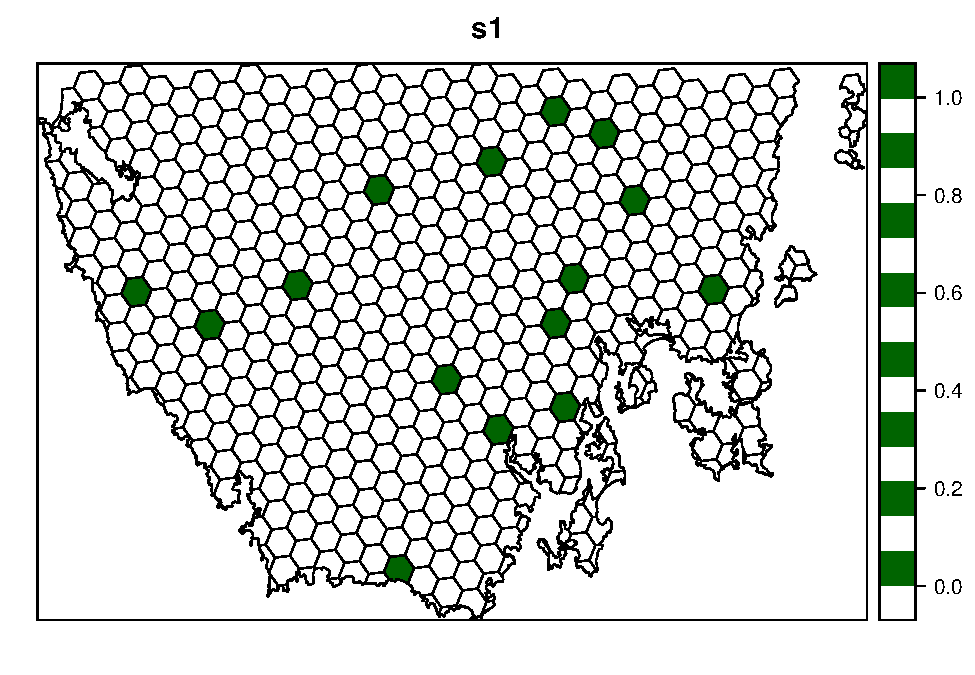
\includegraphics[width=0.65\linewidth]{prioritizr-workshop-manual_files/figure-latex/unnamed-chunk-34-1} \end{center}

Now let's examine the solution.

\begin{rmdquestion}
\begin{enumerate}
\def\labelenumi{\arabic{enumi}.}
\tightlist
\item
  How many planing units were selected in the prioritization? What proportion of planning units were selected in the prioritization?
\item
  Is there a pattern in the spatial distribution of the priority areas?
\item
  Can you verify that all of the targets were met in the prioritization (hint: \texttt{feature\_representation(p1,\ s1{[},\ "solution\_1"{]})})?
\end{enumerate}
\end{rmdquestion}

\hypertarget{adding-complexity}{%
\section{Adding complexity}\label{adding-complexity}}

Our first prioritization suffers many limitations, so let's add additional constraints to the problem to make it more useful. First, let's lock in planing units that are already by covered protected areas. If some vegetation communities are already secured inside existing protected areas, then we might not need to add as many new protected areas to the existing protected area system to meet their targets. Since our planning unit data (\texttt{pu\_da}) already contains this information in the \texttt{locked\_in} column, we can use this column name to specify which planning units should be locked in.

\begin{Shaded}
\begin{Highlighting}[]
\CommentTok{# make prioritization problem}
\NormalTok{p2 <-}\StringTok{ }\KeywordTok{problem}\NormalTok{(pu_data, veg_data, }\DataTypeTok{cost_column =} \StringTok{"cost"}\NormalTok{) }\OperatorTok
\StringTok{      }\KeywordTok{add_min_set_objective}\NormalTok{() }\OperatorTok
\StringTok{      }\KeywordTok{add_relative_targets}\NormalTok{(}\FloatTok{0.05}\NormalTok{) }\OperatorTok
\StringTok{      }\KeywordTok{add_locked_in_constraints}\NormalTok{(}\StringTok{"locked_in"}\NormalTok{) }\OperatorTok
\StringTok{      }\KeywordTok{add_binary_decisions}\NormalTok{() }\OperatorTok
\StringTok{      }\KeywordTok{add_lpsymphony_solver}\NormalTok{(}\DataTypeTok{verbose =} \OtherTok{FALSE}\NormalTok{)}
\end{Highlighting}
\end{Shaded}

\begin{verbatim}
## Warning: Support for sp package will be deprecated.
## i Use `sf::st_as_sf()` to convert data for future compatibility.
\end{verbatim}

\begin{verbatim}
## Warning: Support for raster package will be deprecated.
## i Use `terra::rast()` to convert data for future compatibility.
\end{verbatim}

\begin{Shaded}
\begin{Highlighting}[]
\CommentTok{# print problem}
\KeywordTok{print}\NormalTok{(p2)}
\end{Highlighting}
\end{Shaded}

\begin{verbatim}
## A conservation problem (<ConservationProblem>)
\end{verbatim}

\begin{verbatim}
## +@data
\end{verbatim}

\begin{verbatim}
## |+@features:    "vegetation_1", "vegetation_2", "vegetation_3", "vegetation_4" , ... (32 total)
\end{verbatim}

\begin{verbatim}
## |\@planning units:
\end{verbatim}

\begin{verbatim}
## | +@data:       <SpatialPolygonsDataFrame> (516 total)
\end{verbatim}

\begin{verbatim}
## | +@costs:      continuous values (between 3.5972 and 47.2383)
\end{verbatim}

\begin{verbatim}
## | +@extent:     348703.1831, 5167774.5993, 611932.4474, 5344516.4109 (xmin, ymin, xmax, ymax)
\end{verbatim}

\begin{verbatim}
## | \@CRS:        WGS 84 / UTM zone 55S
\end{verbatim}

\begin{verbatim}
## +@formulation
\end{verbatim}

\begin{verbatim}
## |+@objective:   minimum set objective
\end{verbatim}

\begin{verbatim}
## |+@penalties:   none specified
\end{verbatim}

\begin{verbatim}
## |+@targets:     relative targets (between 0.05 and 0.05)
\end{verbatim}

\begin{verbatim}
## |+@constraints:
\end{verbatim}

\begin{verbatim}
## ||\@1:          locked in constraints (198 planning units)
\end{verbatim}

\begin{verbatim}
## |\@decisions:   binary decision
\end{verbatim}

\begin{verbatim}
## \@optimization
\end{verbatim}

\begin{verbatim}
##  +@portfolio:   shuffle portfolio (`number_solutions` = 1, ...)
\end{verbatim}

\begin{verbatim}
##  \@solver:      lpsymphony (`gap` = 0.1, `time_limit` = 2147483647, `first_feasible` = FALSE, ...)
\end{verbatim}

\begin{verbatim}
## # i Use `summary(...)` to see complete formulation.
\end{verbatim}

\begin{Shaded}
\begin{Highlighting}[]
\CommentTok{# solve problem}
\NormalTok{s2 <-}\StringTok{ }\KeywordTok{solve}\NormalTok{(p2)}

\CommentTok{# plot solution}
\KeywordTok{spplot}\NormalTok{(s2, }\StringTok{"solution_1"}\NormalTok{, }\DataTypeTok{col.regions =} \KeywordTok{c}\NormalTok{(}\StringTok{"white"}\NormalTok{, }\StringTok{"darkgreen"}\NormalTok{), }\DataTypeTok{main =} \StringTok{"s2"}\NormalTok{)}
\end{Highlighting}
\end{Shaded}

\begin{center}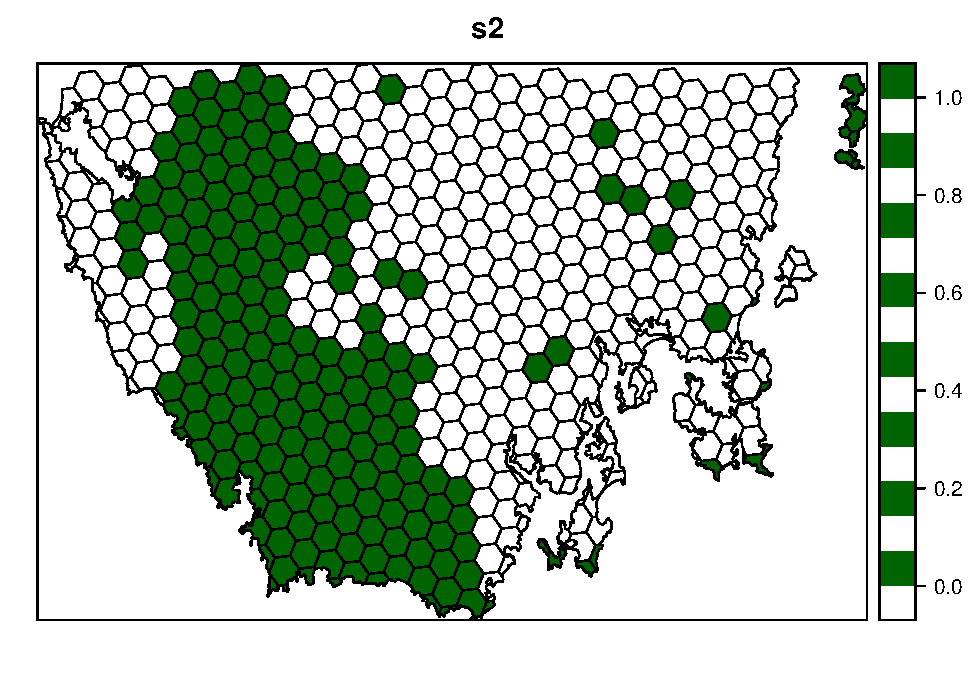
\includegraphics[width=0.65\linewidth]{prioritizr-workshop-manual_files/figure-latex/unnamed-chunk-36-1} \end{center}

Let's pretend that we talked to an expert on the vegetation communities in our study system and they recommended that a 20\% target was needed for each vegetation class. So, armed with this information, let's set the targets to 20\%.

\begin{Shaded}
\begin{Highlighting}[]
\CommentTok{# make prioritization problem}
\NormalTok{p3 <-}\StringTok{ }\KeywordTok{problem}\NormalTok{(pu_data, veg_data, }\DataTypeTok{cost_column =} \StringTok{"cost"}\NormalTok{) }\OperatorTok
\StringTok{      }\KeywordTok{add_min_set_objective}\NormalTok{() }\OperatorTok
\StringTok{      }\KeywordTok{add_relative_targets}\NormalTok{(}\FloatTok{0.2}\NormalTok{) }\OperatorTok
\StringTok{      }\KeywordTok{add_locked_in_constraints}\NormalTok{(}\StringTok{"locked_in"}\NormalTok{) }\OperatorTok
\StringTok{      }\KeywordTok{add_binary_decisions}\NormalTok{() }\OperatorTok
\StringTok{      }\KeywordTok{add_lpsymphony_solver}\NormalTok{(}\DataTypeTok{verbose =} \OtherTok{FALSE}\NormalTok{)}
\end{Highlighting}
\end{Shaded}

\begin{verbatim}
## Warning: Support for sp package will be deprecated.
## i Use `sf::st_as_sf()` to convert data for future compatibility.
\end{verbatim}

\begin{verbatim}
## Warning: Support for raster package will be deprecated.
## i Use `terra::rast()` to convert data for future compatibility.
\end{verbatim}

\begin{Shaded}
\begin{Highlighting}[]
\CommentTok{# print problem}
\KeywordTok{print}\NormalTok{(p3)}
\end{Highlighting}
\end{Shaded}

\begin{verbatim}
## A conservation problem (<ConservationProblem>)
\end{verbatim}

\begin{verbatim}
## +@data
\end{verbatim}

\begin{verbatim}
## |+@features:    "vegetation_1", "vegetation_2", "vegetation_3", "vegetation_4" , ... (32 total)
\end{verbatim}

\begin{verbatim}
## |\@planning units:
\end{verbatim}

\begin{verbatim}
## | +@data:       <SpatialPolygonsDataFrame> (516 total)
\end{verbatim}

\begin{verbatim}
## | +@costs:      continuous values (between 3.5972 and 47.2383)
\end{verbatim}

\begin{verbatim}
## | +@extent:     348703.1831, 5167774.5993, 611932.4474, 5344516.4109 (xmin, ymin, xmax, ymax)
\end{verbatim}

\begin{verbatim}
## | \@CRS:        WGS 84 / UTM zone 55S
\end{verbatim}

\begin{verbatim}
## +@formulation
\end{verbatim}

\begin{verbatim}
## |+@objective:   minimum set objective
\end{verbatim}

\begin{verbatim}
## |+@penalties:   none specified
\end{verbatim}

\begin{verbatim}
## |+@targets:     relative targets (between 0.2 and 0.2)
\end{verbatim}

\begin{verbatim}
## |+@constraints:
\end{verbatim}

\begin{verbatim}
## ||\@1:          locked in constraints (198 planning units)
\end{verbatim}

\begin{verbatim}
## |\@decisions:   binary decision
\end{verbatim}

\begin{verbatim}
## \@optimization
\end{verbatim}

\begin{verbatim}
##  +@portfolio:   shuffle portfolio (`number_solutions` = 1, ...)
\end{verbatim}

\begin{verbatim}
##  \@solver:      lpsymphony (`gap` = 0.1, `time_limit` = 2147483647, `first_feasible` = FALSE, ...)
\end{verbatim}

\begin{verbatim}
## # i Use `summary(...)` to see complete formulation.
\end{verbatim}

\begin{Shaded}
\begin{Highlighting}[]
\CommentTok{# solve problem}
\NormalTok{s3 <-}\StringTok{ }\KeywordTok{solve}\NormalTok{(p3)}

\CommentTok{# plot solution}
\KeywordTok{spplot}\NormalTok{(s3, }\StringTok{"solution_1"}\NormalTok{, }\DataTypeTok{col.regions =} \KeywordTok{c}\NormalTok{(}\StringTok{"white"}\NormalTok{, }\StringTok{"darkgreen"}\NormalTok{), }\DataTypeTok{main =} \StringTok{"s3"}\NormalTok{)}
\end{Highlighting}
\end{Shaded}

\begin{center}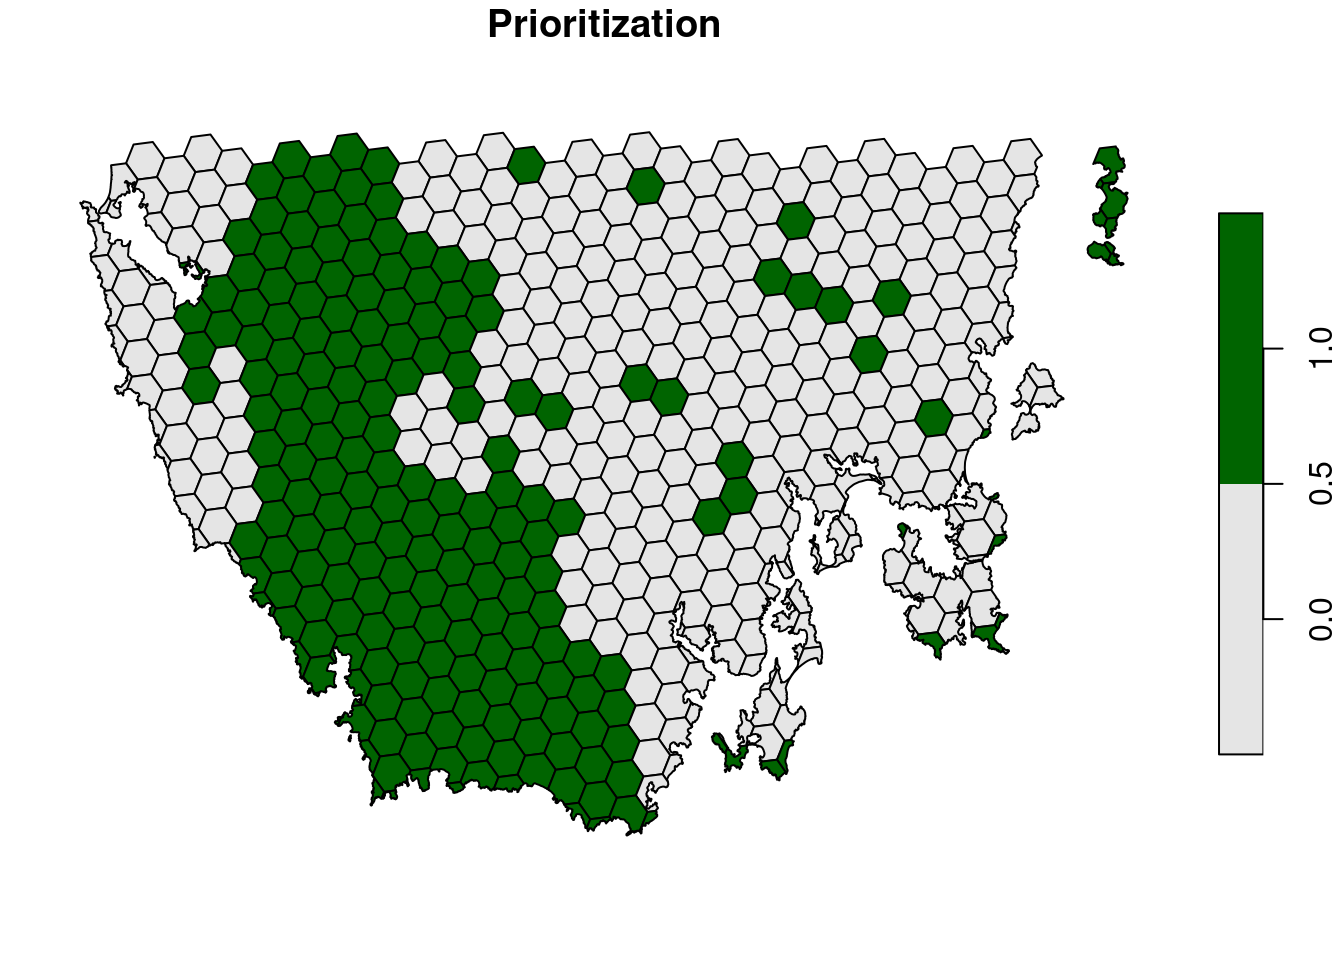
\includegraphics[width=0.65\linewidth]{prioritizr-workshop-manual_files/figure-latex/unnamed-chunk-37-1} \end{center}

Next, let's lock out highly degraded areas. Similar to before, this data is present in our planning unit data so we can use the \texttt{locked\_out} column name to achieve this.

\begin{Shaded}
\begin{Highlighting}[]
\CommentTok{# make prioritization problem}
\NormalTok{p4 <-}\StringTok{ }\KeywordTok{problem}\NormalTok{(pu_data, veg_data, }\DataTypeTok{cost_column =} \StringTok{"cost"}\NormalTok{) }\OperatorTok
\StringTok{      }\KeywordTok{add_min_set_objective}\NormalTok{() }\OperatorTok
\StringTok{      }\KeywordTok{add_relative_targets}\NormalTok{(}\FloatTok{0.1}\NormalTok{) }\OperatorTok
\StringTok{      }\KeywordTok{add_locked_in_constraints}\NormalTok{(}\StringTok{"locked_in"}\NormalTok{) }\OperatorTok
\StringTok{      }\KeywordTok{add_locked_out_constraints}\NormalTok{(}\StringTok{"locked_out"}\NormalTok{) }\OperatorTok
\StringTok{      }\KeywordTok{add_binary_decisions}\NormalTok{() }\OperatorTok
\StringTok{      }\KeywordTok{add_lpsymphony_solver}\NormalTok{(}\DataTypeTok{verbose =} \OtherTok{FALSE}\NormalTok{)}
\end{Highlighting}
\end{Shaded}

\begin{verbatim}
## Warning: Support for sp package will be deprecated.
## i Use `sf::st_as_sf()` to convert data for future compatibility.
\end{verbatim}

\begin{verbatim}
## Warning: Support for raster package will be deprecated.
## i Use `terra::rast()` to convert data for future compatibility.
\end{verbatim}

\begin{Shaded}
\begin{Highlighting}[]
\CommentTok{# print problem}
\KeywordTok{print}\NormalTok{(p4)}
\end{Highlighting}
\end{Shaded}

\begin{verbatim}
## A conservation problem (<ConservationProblem>)
\end{verbatim}

\begin{verbatim}
## +@data
\end{verbatim}

\begin{verbatim}
## |+@features:    "vegetation_1", "vegetation_2", "vegetation_3", "vegetation_4" , ... (32 total)
\end{verbatim}

\begin{verbatim}
## |\@planning units:
\end{verbatim}

\begin{verbatim}
## | +@data:       <SpatialPolygonsDataFrame> (516 total)
\end{verbatim}

\begin{verbatim}
## | +@costs:      continuous values (between 3.5972 and 47.2383)
\end{verbatim}

\begin{verbatim}
## | +@extent:     348703.1831, 5167774.5993, 611932.4474, 5344516.4109 (xmin, ymin, xmax, ymax)
\end{verbatim}

\begin{verbatim}
## | \@CRS:        WGS 84 / UTM zone 55S
\end{verbatim}

\begin{verbatim}
## +@formulation
\end{verbatim}

\begin{verbatim}
## |+@objective:   minimum set objective
\end{verbatim}

\begin{verbatim}
## |+@penalties:   none specified
\end{verbatim}

\begin{verbatim}
## |+@targets:     relative targets (between 0.1 and 0.1)
\end{verbatim}

\begin{verbatim}
## |+@constraints:
\end{verbatim}

\begin{verbatim}
## ||+@1:          locked in constraints (198 planning units)
\end{verbatim}

\begin{verbatim}
## ||\@2:          locked out constraints (6 planning units)
\end{verbatim}

\begin{verbatim}
## |\@decisions:   binary decision
\end{verbatim}

\begin{verbatim}
## \@optimization
\end{verbatim}

\begin{verbatim}
##  +@portfolio:   shuffle portfolio (`number_solutions` = 1, ...)
\end{verbatim}

\begin{verbatim}
##  \@solver:      lpsymphony (`gap` = 0.1, `time_limit` = 2147483647, `first_feasible` = FALSE, ...)
\end{verbatim}

\begin{verbatim}
## # i Use `summary(...)` to see complete formulation.
\end{verbatim}

\begin{Shaded}
\begin{Highlighting}[]
\CommentTok{# solve problem}
\NormalTok{s4 <-}\StringTok{ }\KeywordTok{solve}\NormalTok{(p4)}

\CommentTok{# plot solution}
\KeywordTok{spplot}\NormalTok{(s4, }\StringTok{"solution_1"}\NormalTok{, }\DataTypeTok{col.regions =} \KeywordTok{c}\NormalTok{(}\StringTok{"white"}\NormalTok{, }\StringTok{"darkgreen"}\NormalTok{), }\DataTypeTok{main =} \StringTok{"s4"}\NormalTok{)}
\end{Highlighting}
\end{Shaded}

\begin{center}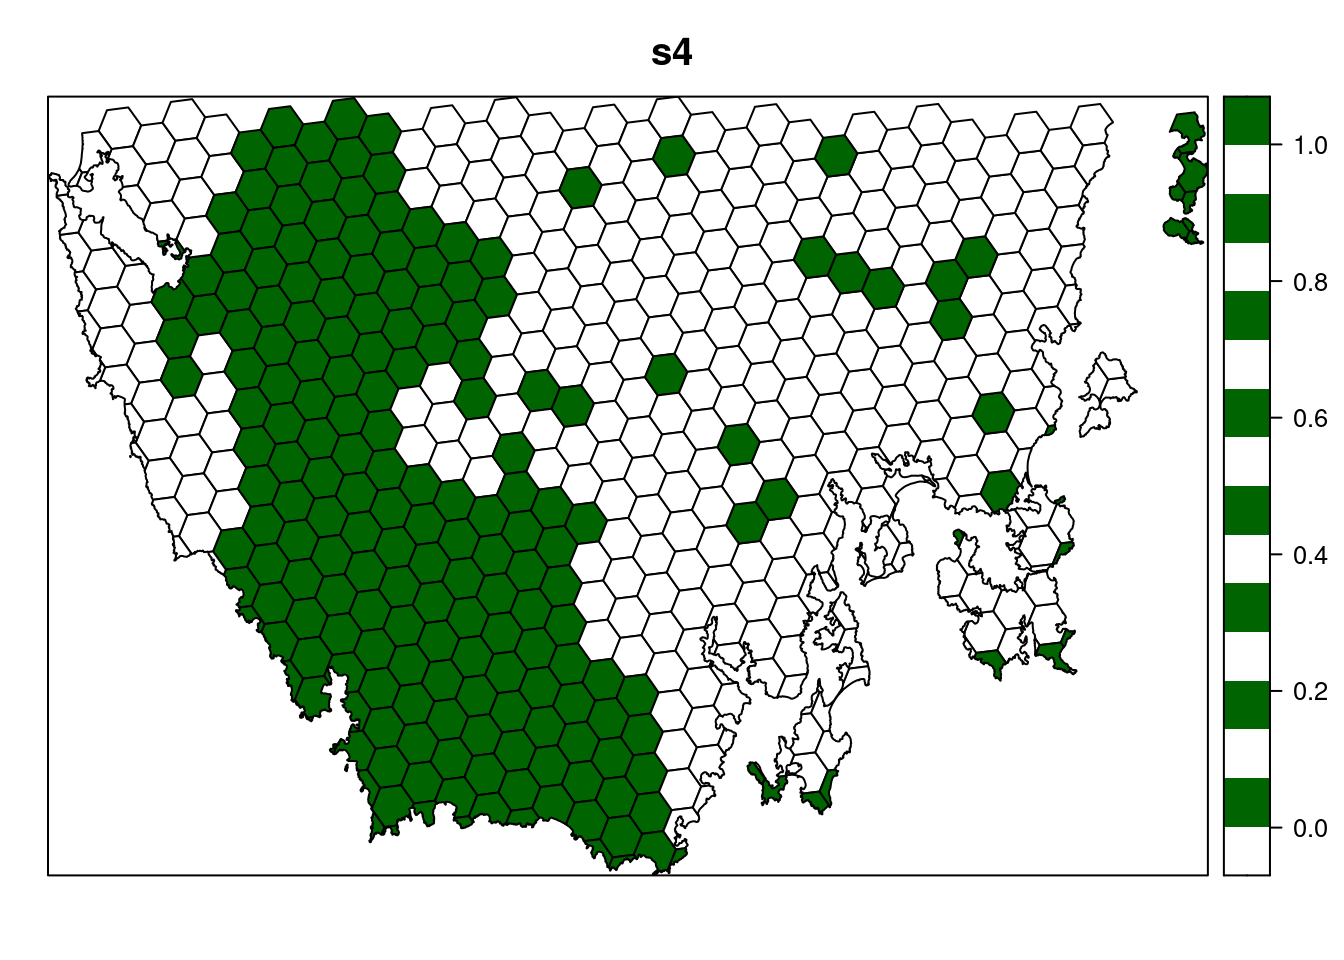
\includegraphics[width=0.65\linewidth]{prioritizr-workshop-manual_files/figure-latex/unnamed-chunk-39-1} \end{center}

\clearpage

Now, let's compare the solutions.

\begin{rmdquestion}
\begin{enumerate}
\def\labelenumi{\arabic{enumi}.}
\tightlist
\item
  What is the cost of the planning units selected in \texttt{s2}, \texttt{s3}, and \texttt{s4}?
\item
  How many planning units are in \texttt{s2}, \texttt{s3}, and \texttt{s4}?
\item
  Do the solutions with more planning units have a greater cost? Why or why not?
\item
  Why does the first solution (\texttt{s1}) cost less than the second solution with protected areas locked into the solution (\texttt{s2})?
\item
  Why does the third solution (\texttt{s3}) cost less than the fourth solution solution with highly degraded areas locked out (\texttt{s4})?
\item
  Since planning units covered by existing protected areas have already been purchased, what is the cost for expanding the protected area system based on on the fourth prioritization (\texttt{s4}) (hint: total cost minus the cost of locked in planning units)?
\item
  What happens if you specify targets that exceed the total amount of vegetation in the study area and try to solve the problem? You can do this by modifying the code to make \texttt{p4} with \texttt{add\_absolute\_targets(1000)} instead of \texttt{add\_relative\_targets(0.2)} and generating a new solution.
\end{enumerate}
\end{rmdquestion}

\hypertarget{penalizing-fragmentation}{%
\section{Penalizing fragmentation}\label{penalizing-fragmentation}}

Plans for protected area systems should facilitate gene flow and dispersal between individual reserves in the system. However, the prioritizations we have made so far have been highly fragmented. Similar to the Marxan decision support tool, we can add penalties to our conservation planning problem to penalize fragmentation (i.e.~total exposed boundary length) and we also need to set a useful penalty value when adding such penalties (akin to Marxan's boundary length multiplier value; BLM). If we set our penalty value too low, then we will end up with a solution that is identical to the solution with no added penalties. If we set our penalty value too high, then prioritizr will take a long time to solve the problem and we will end up with a solution that contains lots of extra planning units that are not needed (since the penalty value is so high that minimizing fragmentation is more important than cost). As a rule of thumb, we generally want penalty values between 0.00001 and 0.01 but finding a useful penalty value requires calibration. The ``correct'' penalty value depends on the size of the planning units, the main objective values (e.g.~cost values), and the effect of fragmentation on biodiversity persistence. Let's create a new problem that is similar to our previous problem (\texttt{p4})---except that it contains boundary length penalties and a slightly higher optimality gap to reduce runtime (default is 0.1)---and solve it. Since our planning unit data is in a spatial format (i.e.~vector or raster data), prioritizr can automatically calculate the boundary data for us.

\clearpage

\begin{Shaded}
\begin{Highlighting}[]
\CommentTok{# make prioritization problem}
\NormalTok{p5 <-}\StringTok{ }\KeywordTok{problem}\NormalTok{(pu_data, veg_data, }\DataTypeTok{cost_column =} \StringTok{"cost"}\NormalTok{) }\OperatorTok
\StringTok{      }\KeywordTok{add_min_set_objective}\NormalTok{() }\OperatorTok
\StringTok{      }\KeywordTok{add_boundary_penalties}\NormalTok{(}\DataTypeTok{penalty =} \FloatTok{0.0005}\NormalTok{) }\OperatorTok
\StringTok{      }\KeywordTok{add_relative_targets}\NormalTok{(}\FloatTok{0.1}\NormalTok{) }\OperatorTok
\StringTok{      }\KeywordTok{add_locked_in_constraints}\NormalTok{(}\StringTok{"locked_in"}\NormalTok{) }\OperatorTok
\StringTok{      }\KeywordTok{add_locked_out_constraints}\NormalTok{(}\StringTok{"locked_out"}\NormalTok{) }\OperatorTok
\StringTok{      }\KeywordTok{add_binary_decisions}\NormalTok{() }\OperatorTok
\StringTok{      }\KeywordTok{add_lpsymphony_solver}\NormalTok{(}\DataTypeTok{verbose =} \OtherTok{FALSE}\NormalTok{, }\DataTypeTok{gap =} \DecValTok{1}\NormalTok{)}
\end{Highlighting}
\end{Shaded}

\begin{verbatim}
## Warning: Support for sp package will be deprecated.
## i Use `sf::st_as_sf()` to convert data for future compatibility.
\end{verbatim}

\begin{verbatim}
## Warning: Support for raster package will be deprecated.
## i Use `terra::rast()` to convert data for future compatibility.
\end{verbatim}

\begin{Shaded}
\begin{Highlighting}[]
\CommentTok{# print problem}
\KeywordTok{print}\NormalTok{(p5)}
\end{Highlighting}
\end{Shaded}

\begin{verbatim}
## A conservation problem (<ConservationProblem>)
\end{verbatim}

\begin{verbatim}
## +@data
\end{verbatim}

\begin{verbatim}
## |+@features:    "vegetation_1", "vegetation_2", "vegetation_3", "vegetation_4" , ... (32 total)
\end{verbatim}

\begin{verbatim}
## |\@planning units:
\end{verbatim}

\begin{verbatim}
## | +@data:       <SpatialPolygonsDataFrame> (516 total)
\end{verbatim}

\begin{verbatim}
## | +@costs:      continuous values (between 3.5972 and 47.2383)
\end{verbatim}

\begin{verbatim}
## | +@extent:     348703.1831, 5167774.5993, 611932.4474, 5344516.4109 (xmin, ymin, xmax, ymax)
\end{verbatim}

\begin{verbatim}
## | \@CRS:        WGS 84 / UTM zone 55S
\end{verbatim}

\begin{verbatim}
## +@formulation
\end{verbatim}

\begin{verbatim}
## |+@objective:   minimum set objective
\end{verbatim}

\begin{verbatim}
## |+@penalties:
\end{verbatim}

\begin{verbatim}
## ||\@1:          boundary penalties (`penalty` = 5e-04, `edge_factor` = 0.5, ...)
\end{verbatim}

\begin{verbatim}
## |+@targets:     relative targets (between 0.1 and 0.1)
\end{verbatim}

\begin{verbatim}
## |+@constraints:
\end{verbatim}

\begin{verbatim}
## ||+@1:          locked in constraints (198 planning units)
\end{verbatim}

\begin{verbatim}
## ||\@2:          locked out constraints (6 planning units)
\end{verbatim}

\begin{verbatim}
## |\@decisions:   binary decision
\end{verbatim}

\begin{verbatim}
## \@optimization
\end{verbatim}

\begin{verbatim}
##  +@portfolio:   shuffle portfolio (`number_solutions` = 1, ...)
\end{verbatim}

\begin{verbatim}
##  \@solver:      lpsymphony (`gap` = 1, `time_limit` = 2147483647, `first_feasible` = FALSE, ...)
\end{verbatim}

\begin{verbatim}
## # i Use `summary(...)` to see complete formulation.
\end{verbatim}

\begin{Shaded}
\begin{Highlighting}[]
\CommentTok{# solve problem,}
\CommentTok{# note this will take around 30 seconds}
\NormalTok{s5 <-}\StringTok{ }\KeywordTok{solve}\NormalTok{(p5)}
\end{Highlighting}
\end{Shaded}

\begin{verbatim}
## Warning: Support for sp package will be deprecated.
## i Use `sf::st_as_sf()` to convert data for future compatibility.
\end{verbatim}

\begin{Shaded}
\begin{Highlighting}[]
\CommentTok{# print solution}
\KeywordTok{print}\NormalTok{(s5)}
\end{Highlighting}
\end{Shaded}

\begin{verbatim}
## class       : SpatialPolygonsDataFrame 
## features    : 516 
## extent      : 348703.2, 611932.4, 5167775, 5344516  (xmin, xmax, ymin, ymax)
## crs         : +proj=utm +zone=55 +south +datum=WGS84 +units=m +no_defs 
## variables   : 7
## names       :   id,             cost, status, locked_in, locked_out, pa_status, solution_1 
## min values  :  557, 3.59717531470679,      0,         0,          0,         0,          0 
## max values  : 1130,  47.238336402701,      2,         1,          1,         1,          1
\end{verbatim}

\begin{Shaded}
\begin{Highlighting}[]
\CommentTok{# plot solution}
\KeywordTok{spplot}\NormalTok{(s5, }\StringTok{"solution_1"}\NormalTok{, }\DataTypeTok{col.regions =} \KeywordTok{c}\NormalTok{(}\StringTok{"white"}\NormalTok{, }\StringTok{"darkgreen"}\NormalTok{), }\DataTypeTok{main =} \StringTok{"s5"}\NormalTok{)}
\end{Highlighting}
\end{Shaded}

\begin{center}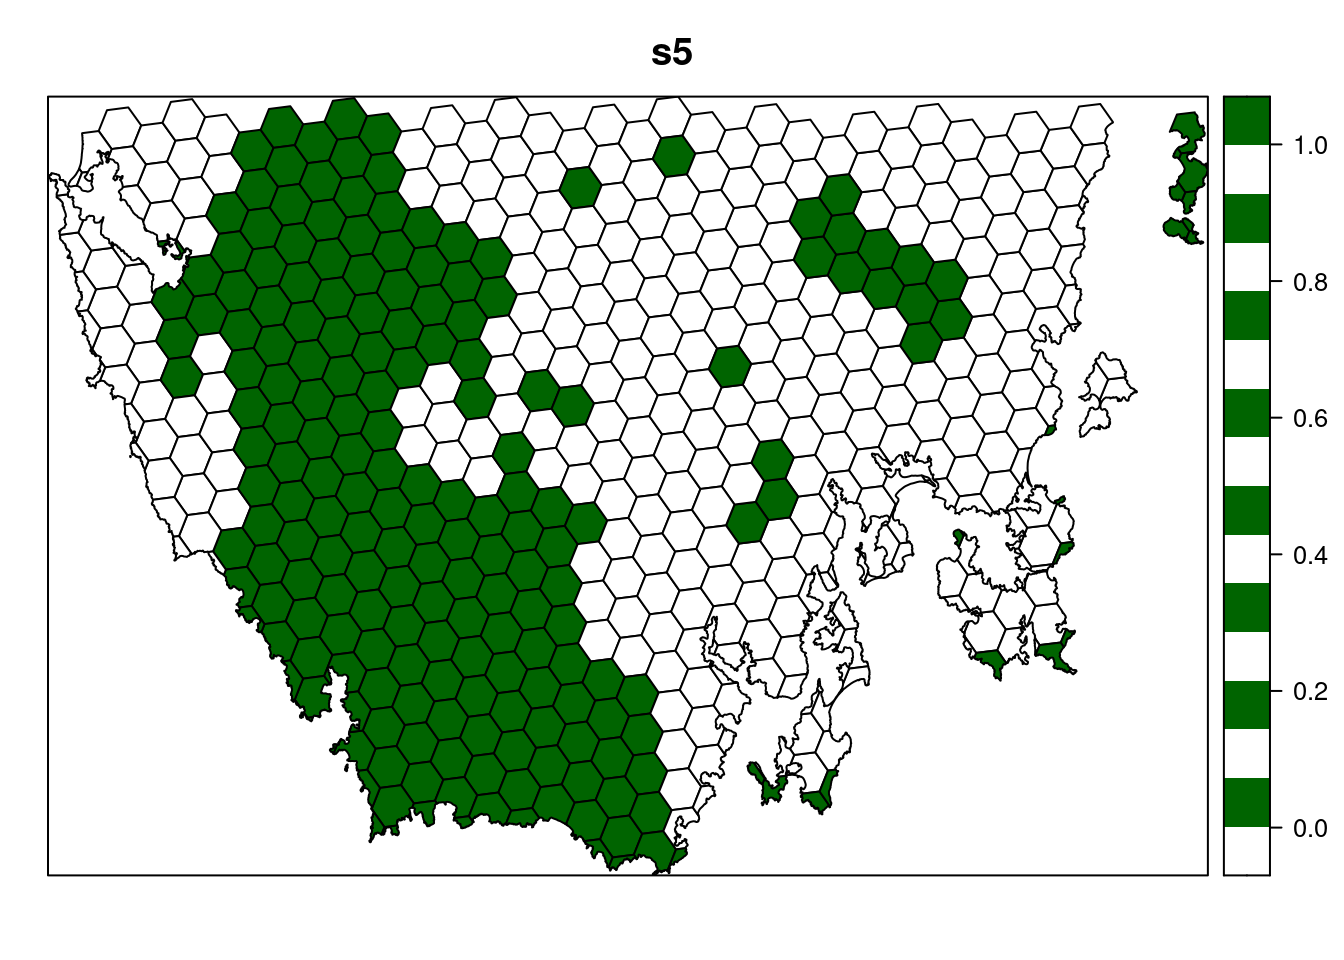
\includegraphics[width=0.65\linewidth]{prioritizr-workshop-manual_files/figure-latex/unnamed-chunk-41-1} \end{center}

Now let's compare the solutions to the problems with (\texttt{s5}) and without (\texttt{s4}) the boundary length penalties.

\begin{rmdquestion}
\begin{enumerate}
\def\labelenumi{\arabic{enumi}.}
\tightlist
\item
  What is the cost the fourth (\texttt{s4}) and fifth (\texttt{s5}) solutions? Why does the fifth solution (\texttt{s5}) cost more than the fourth (\texttt{s4}) solution?
\item
  Try setting the penalty value to 0.000000001 (i.e.~\texttt{1e-9}) instead of 0.0005. What is the cost of the solution now? Is it different from the fourth solution (\texttt{s4}) (hint: try plotting the solutions to visualize them)? Is this is a useful penalty value? Why?
\item
  Try setting the penalty value to 0.5. What is the cost of the solution now? Is it different from the fourth solution (\texttt{s4}) (hint: try plotting the solutions to visualize them)? Is this a useful penalty value? Why?
\end{enumerate}
\end{rmdquestion}

\clearpage

\hypertarget{budget-limited-prioritizations}{%
\section{Budget limited prioritizations}\label{budget-limited-prioritizations}}

In the real-world, the funding available for conservation is often very limited. As a consequence, decision makers often need prioritizations where the total cost of priority areas does not exceed a budget. In our fourth prioritization (\texttt{s4}), we found that we would need to spend an additional \$226 million AUD to ensure that each vegetation community is adequately represented in the protected area system. But what if the funds available for establishing new protected areas were limited to \$100 million AUD? In this case, we need a ``budget limited prioritization''. Budget limited prioritizations aim to maximize some measure of conservation benefit subject to a budget (e.g.~\href{https://prioritizr.net/reference/add_max_cover_objective.html}{number of species with at least one occurrence in the protected area system}, or \href{https://prioritizr.net/reference/add_max_phylo_div_objective.html}{phylogenetic diversity}). Let's create a prioritization by maximizing the number of adequately represented features whilst keeping within a pre-specified budget.

\begin{Shaded}
\begin{Highlighting}[]
\CommentTok{# funds for additional land acquisition (same units as cost data)}
\NormalTok{funds <-}\StringTok{ }\DecValTok{100}

\CommentTok{# calculate the total budget for the prioritization}
\NormalTok{budget <-}\StringTok{ }\NormalTok{funds }\OperatorTok{+}\StringTok{ }\KeywordTok{sum}\NormalTok{(s4}\OperatorTok{$}\NormalTok{cost }\OperatorTok{*}\StringTok{ }\NormalTok{s4}\OperatorTok{$}\NormalTok{locked_in)}
\KeywordTok{print}\NormalTok{(budget)}
\end{Highlighting}
\end{Shaded}

\begin{verbatim}
## [1] 6580.64
\end{verbatim}

\begin{Shaded}
\begin{Highlighting}[]
\CommentTok{# make prioritization problem}
\NormalTok{p6 <-}\StringTok{ }\KeywordTok{problem}\NormalTok{(pu_data, veg_data, }\DataTypeTok{cost_column =} \StringTok{"cost"}\NormalTok{) }\OperatorTok
\StringTok{      }\KeywordTok{add_max_features_objective}\NormalTok{(budget) }\OperatorTok
\StringTok{      }\KeywordTok{add_relative_targets}\NormalTok{(}\FloatTok{0.1}\NormalTok{) }\OperatorTok
\StringTok{      }\KeywordTok{add_locked_in_constraints}\NormalTok{(}\StringTok{"locked_in"}\NormalTok{) }\OperatorTok
\StringTok{      }\KeywordTok{add_locked_out_constraints}\NormalTok{(}\StringTok{"locked_out"}\NormalTok{) }\OperatorTok
\StringTok{      }\KeywordTok{add_binary_decisions}\NormalTok{() }\OperatorTok
\StringTok{      }\KeywordTok{add_lpsymphony_solver}\NormalTok{(}\DataTypeTok{verbose =} \OtherTok{FALSE}\NormalTok{)}
\end{Highlighting}
\end{Shaded}

\begin{verbatim}
## Warning: Support for sp package will be deprecated.
## i Use `sf::st_as_sf()` to convert data for future compatibility.
\end{verbatim}

\begin{verbatim}
## Warning: Support for raster package will be deprecated.
## i Use `terra::rast()` to convert data for future compatibility.
\end{verbatim}

\begin{Shaded}
\begin{Highlighting}[]
\CommentTok{# print problem}
\KeywordTok{print}\NormalTok{(p6)}
\end{Highlighting}
\end{Shaded}

\begin{verbatim}
## A conservation problem (<ConservationProblem>)
\end{verbatim}

\begin{verbatim}
## +@data
\end{verbatim}

\begin{verbatim}
## |+@features:    "vegetation_1", "vegetation_2", "vegetation_3", "vegetation_4" , ... (32 total)
\end{verbatim}

\begin{verbatim}
## |\@planning units:
\end{verbatim}

\begin{verbatim}
## | +@data:       <SpatialPolygonsDataFrame> (516 total)
\end{verbatim}

\begin{verbatim}
## | +@costs:      continuous values (between 3.5972 and 47.2383)
\end{verbatim}

\begin{verbatim}
## | +@extent:     348703.1831, 5167774.5993, 611932.4474, 5344516.4109 (xmin, ymin, xmax, ymax)
\end{verbatim}

\begin{verbatim}
## | \@CRS:        WGS 84 / UTM zone 55S
\end{verbatim}

\begin{verbatim}
## +@formulation
\end{verbatim}

\begin{verbatim}
## |+@objective:   maximum representation objective (`budget` = 6580.6397)
\end{verbatim}

\begin{verbatim}
## |+@penalties:   none specified
\end{verbatim}

\begin{verbatim}
## |+@targets:     relative targets (between 0.1 and 0.1)
\end{verbatim}

\begin{verbatim}
## |+@constraints:
\end{verbatim}

\begin{verbatim}
## ||+@1:          locked in constraints (198 planning units)
\end{verbatim}

\begin{verbatim}
## ||\@2:          locked out constraints (6 planning units)
\end{verbatim}

\begin{verbatim}
## |\@decisions:   binary decision
\end{verbatim}

\begin{verbatim}
## \@optimization
\end{verbatim}

\begin{verbatim}
##  +@portfolio:   shuffle portfolio (`number_solutions` = 1, ...)
\end{verbatim}

\begin{verbatim}
##  \@solver:      lpsymphony (`gap` = 0.1, `time_limit` = 2147483647, `first_feasible` = FALSE, ...)
\end{verbatim}

\begin{verbatim}
## # i Use `summary(...)` to see complete formulation.
\end{verbatim}

\begin{Shaded}
\begin{Highlighting}[]
\CommentTok{# solve problem}
\NormalTok{s6 <-}\StringTok{ }\KeywordTok{solve}\NormalTok{(p6)}

\CommentTok{# plot solution}
\KeywordTok{spplot}\NormalTok{(s6, }\StringTok{"solution_1"}\NormalTok{, }\DataTypeTok{col.regions =} \KeywordTok{c}\NormalTok{(}\StringTok{"white"}\NormalTok{, }\StringTok{"darkgreen"}\NormalTok{), }\DataTypeTok{main =} \StringTok{"s6"}\NormalTok{)}
\end{Highlighting}
\end{Shaded}

\begin{center}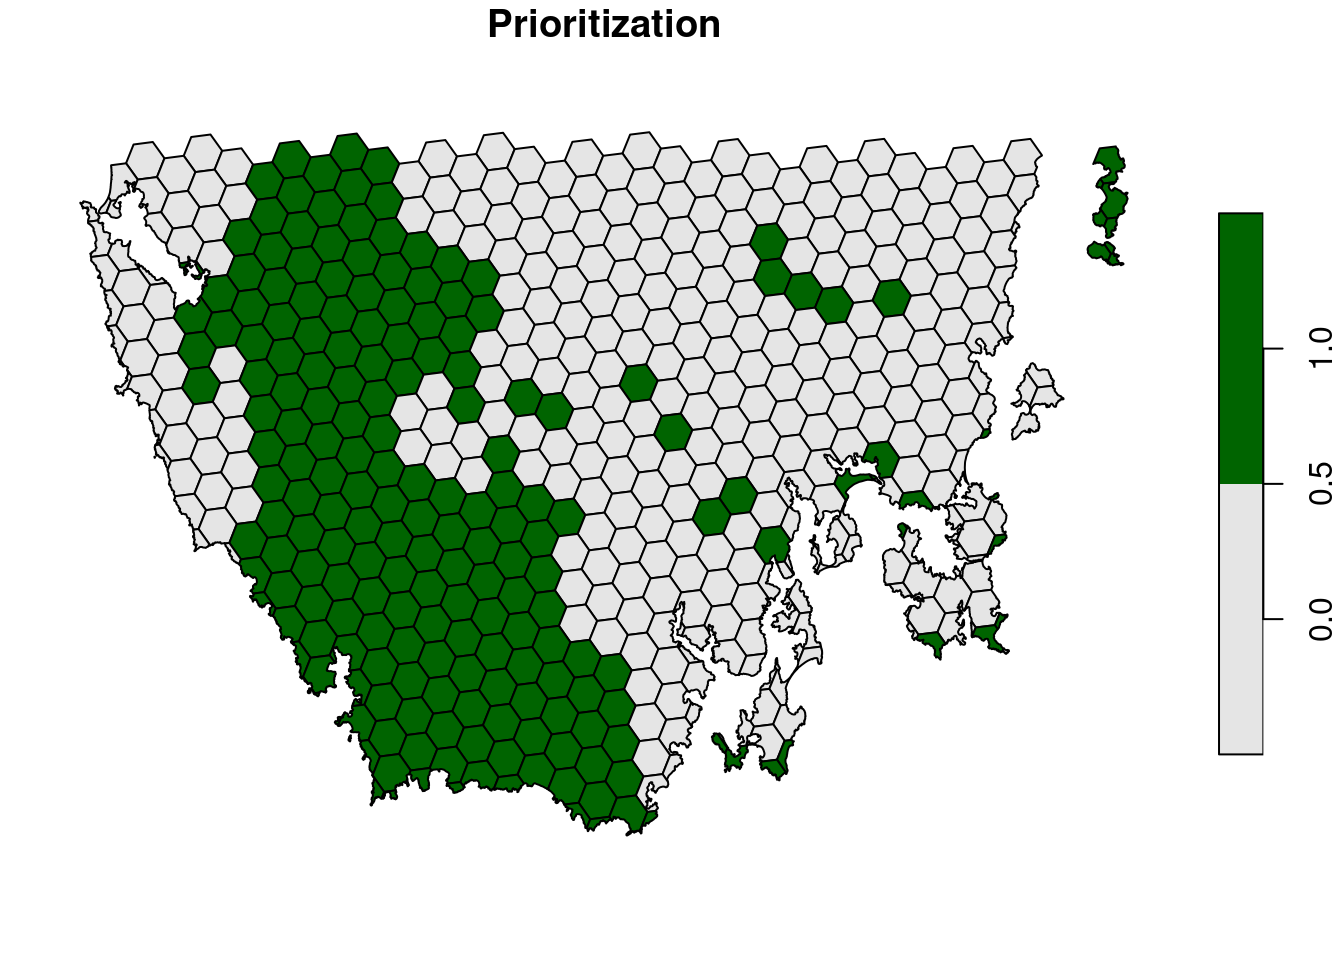
\includegraphics[width=0.65\linewidth]{prioritizr-workshop-manual_files/figure-latex/budget-1} \end{center}

\begin{Shaded}
\begin{Highlighting}[]
\CommentTok{# calculate feature representation}
\NormalTok{r6 <-}\StringTok{ }\KeywordTok{eval_feature_representation_summary}\NormalTok{(p6, s6[, }\StringTok{"solution_1"}\NormalTok{])}
\end{Highlighting}
\end{Shaded}

\begin{verbatim}
## Warning: Support for sp package will be deprecated.
## i Use `sf::st_as_sf()` to convert data for future compatibility.
\end{verbatim}

\begin{Shaded}
\begin{Highlighting}[]
\CommentTok{# calculate number of features with targets met}
\KeywordTok{sum}\NormalTok{(r6}\OperatorTok{$}\NormalTok{relative_held }\OperatorTok{>=}\StringTok{ }\FloatTok{0.2}\NormalTok{, }\DataTypeTok{na.rm =} \OtherTok{TRUE}\NormalTok{)}
\end{Highlighting}
\end{Shaded}

\begin{verbatim}
## [1] 16
\end{verbatim}

\begin{Shaded}
\begin{Highlighting}[]
\CommentTok{# find out which features have their targets met when we add weights,}
\CommentTok{# note that NA is for vegetation.61}
\KeywordTok{print}\NormalTok{(r6}\OperatorTok{$}\NormalTok{feature[r6}\OperatorTok{$}\NormalTok{relative_held }\OperatorTok{>=}\StringTok{ }\FloatTok{0.2}\NormalTok{])}
\end{Highlighting}
\end{Shaded}

\begin{verbatim}
##  [1] "vegetation_4"  "vegetation_5"  "vegetation_14" "vegetation_17"
##  [5] "vegetation_18" "vegetation_19" "vegetation_20" "vegetation_21"
##  [9] "vegetation_22" "vegetation_23" "vegetation_24" "vegetation_25"
## [13] "vegetation_26" "vegetation_27" "vegetation_28" "vegetation_29"
\end{verbatim}

We can also add weights to specify that it is more important to meet the targets for certain features and less important for other features. A common approach for weighting features is to assign a greater importance to features with smaller spatial distributions. The rationale behind this weighting method is that features with smaller spatial distributions are at greater risk of extinction. So, let's calculate some weights for our vegetation communities and see how weighting the features changes our prioritization.

\begin{Shaded}
\begin{Highlighting}[]
\CommentTok{# calculate weights as the log inverse number of grid cells that each vegetation}
\CommentTok{# class occupies, rescaled between 1 and 100}
\NormalTok{wts <-}\StringTok{ }\DecValTok{1} \OperatorTok{/}\StringTok{ }\KeywordTok{cellStats}\NormalTok{(veg_data, }\StringTok{"sum"}\NormalTok{)}
\NormalTok{wts <-}\StringTok{ }\KeywordTok{rescale}\NormalTok{(wts, }\DataTypeTok{to =} \KeywordTok{c}\NormalTok{(}\DecValTok{1}\NormalTok{, }\DecValTok{10}\NormalTok{))}

\CommentTok{# print the name of the feature with smallest weight}
\KeywordTok{names}\NormalTok{(veg_data)[}\KeywordTok{which.min}\NormalTok{(wts)]}
\end{Highlighting}
\end{Shaded}

\begin{verbatim}
## [1] "vegetation_12"
\end{verbatim}

\begin{Shaded}
\begin{Highlighting}[]
\CommentTok{# print the name of the feature with greatest weight}
\KeywordTok{names}\NormalTok{(veg_data)[}\KeywordTok{which.max}\NormalTok{(wts)]}
\end{Highlighting}
\end{Shaded}

\begin{verbatim}
## [1] "vegetation_3"
\end{verbatim}

\begin{Shaded}
\begin{Highlighting}[]
\CommentTok{# plot histogram of weights}
\KeywordTok{hist}\NormalTok{(wts, }\DataTypeTok{main =} \StringTok{"feature weights"}\NormalTok{)}
\end{Highlighting}
\end{Shaded}

\begin{center}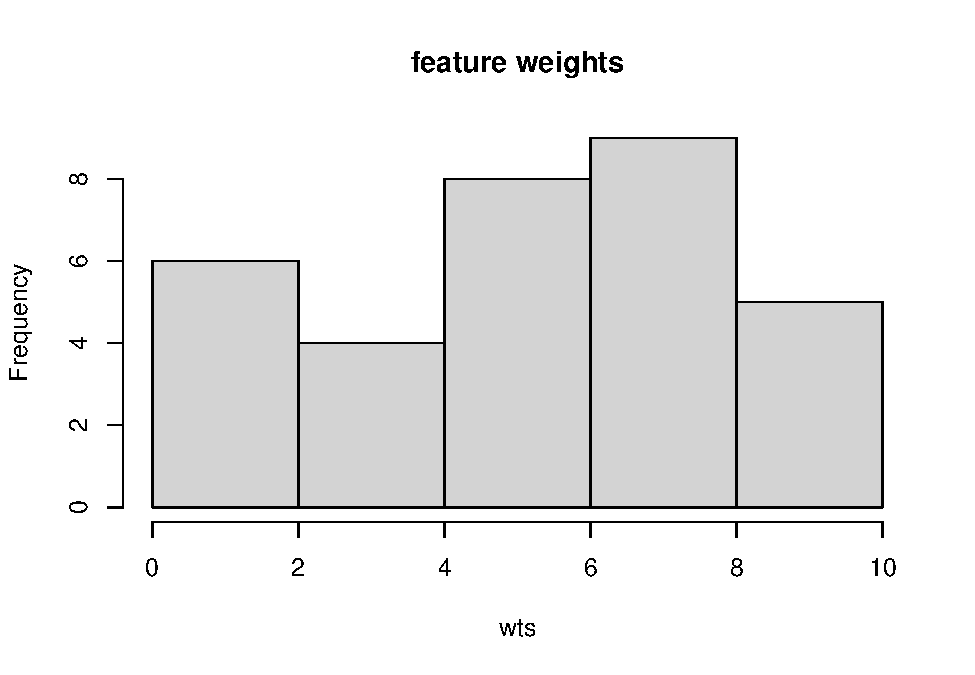
\includegraphics[width=0.65\linewidth]{prioritizr-workshop-manual_files/figure-latex/budget-weights-1} \end{center}

\begin{Shaded}
\begin{Highlighting}[]
\CommentTok{# make prioritization problem with weights}
\NormalTok{p7 <-}\StringTok{ }\KeywordTok{problem}\NormalTok{(pu_data, veg_data, }\DataTypeTok{cost_column =} \StringTok{"cost"}\NormalTok{) }\OperatorTok
\StringTok{      }\KeywordTok{add_max_features_objective}\NormalTok{(budget) }\OperatorTok
\StringTok{      }\KeywordTok{add_relative_targets}\NormalTok{(}\FloatTok{0.1}\NormalTok{) }\OperatorTok
\StringTok{      }\KeywordTok{add_feature_weights}\NormalTok{(wts) }\OperatorTok
\StringTok{      }\KeywordTok{add_locked_in_constraints}\NormalTok{(}\StringTok{"locked_in"}\NormalTok{) }\OperatorTok
\StringTok{      }\KeywordTok{add_locked_out_constraints}\NormalTok{(}\StringTok{"locked_out"}\NormalTok{) }\OperatorTok
\StringTok{      }\KeywordTok{add_binary_decisions}\NormalTok{() }\OperatorTok
\StringTok{      }\KeywordTok{add_lpsymphony_solver}\NormalTok{(}\DataTypeTok{verbose =} \OtherTok{FALSE}\NormalTok{)}
\end{Highlighting}
\end{Shaded}

\begin{verbatim}
## Warning: Support for sp package will be deprecated.
## i Use `sf::st_as_sf()` to convert data for future compatibility.
\end{verbatim}

\begin{verbatim}
## Warning: Support for raster package will be deprecated.
## i Use `terra::rast()` to convert data for future compatibility.
\end{verbatim}

\begin{Shaded}
\begin{Highlighting}[]
\CommentTok{# print problem}
\KeywordTok{print}\NormalTok{(p7)}
\end{Highlighting}
\end{Shaded}

\begin{verbatim}
## A conservation problem (<ConservationProblem>)
\end{verbatim}

\begin{verbatim}
## +@data
\end{verbatim}

\begin{verbatim}
## |+@features:    "vegetation_1", "vegetation_2", "vegetation_3", "vegetation_4" , ... (32 total)
\end{verbatim}

\begin{verbatim}
## |\@planning units:
\end{verbatim}

\begin{verbatim}
## | +@data:       <SpatialPolygonsDataFrame> (516 total)
\end{verbatim}

\begin{verbatim}
## | +@costs:      continuous values (between 3.5972 and 47.2383)
\end{verbatim}

\begin{verbatim}
## | +@extent:     348703.1831, 5167774.5993, 611932.4474, 5344516.4109 (xmin, ymin, xmax, ymax)
\end{verbatim}

\begin{verbatim}
## | \@CRS:        WGS 84 / UTM zone 55S
\end{verbatim}

\begin{verbatim}
## +@formulation
\end{verbatim}

\begin{verbatim}
## |+@objective:   maximum representation objective (`budget` = 6580.6397)
\end{verbatim}

\begin{verbatim}
## |+@penalties:
\end{verbatim}

\begin{verbatim}
## ||\@1:          feature weights (`weights` = asymmetric continuous values (non-zero values between 1 and 10))
\end{verbatim}

\begin{verbatim}
## |+@targets:     relative targets (between 0.1 and 0.1)
\end{verbatim}

\begin{verbatim}
## |+@constraints:
\end{verbatim}

\begin{verbatim}
## ||+@1:          locked in constraints (198 planning units)
\end{verbatim}

\begin{verbatim}
## ||\@2:          locked out constraints (6 planning units)
\end{verbatim}

\begin{verbatim}
## |\@decisions:   binary decision
\end{verbatim}

\begin{verbatim}
## \@optimization
\end{verbatim}

\begin{verbatim}
##  +@portfolio:   shuffle portfolio (`number_solutions` = 1, ...)
\end{verbatim}

\begin{verbatim}
##  \@solver:      lpsymphony (`gap` = 0.1, `time_limit` = 2147483647, `first_feasible` = FALSE, ...)
\end{verbatim}

\begin{verbatim}
## # i Use `summary(...)` to see complete formulation.
\end{verbatim}

\begin{Shaded}
\begin{Highlighting}[]
\CommentTok{# solve problem}
\NormalTok{s7 <-}\StringTok{ }\KeywordTok{solve}\NormalTok{(p7)}

\CommentTok{# plot solution}
\KeywordTok{spplot}\NormalTok{(s7, }\StringTok{"solution_1"}\NormalTok{, }\DataTypeTok{col.regions =} \KeywordTok{c}\NormalTok{(}\StringTok{"white"}\NormalTok{, }\StringTok{"darkgreen"}\NormalTok{), }\DataTypeTok{main =} \StringTok{"s7"}\NormalTok{)}
\end{Highlighting}
\end{Shaded}

\begin{center}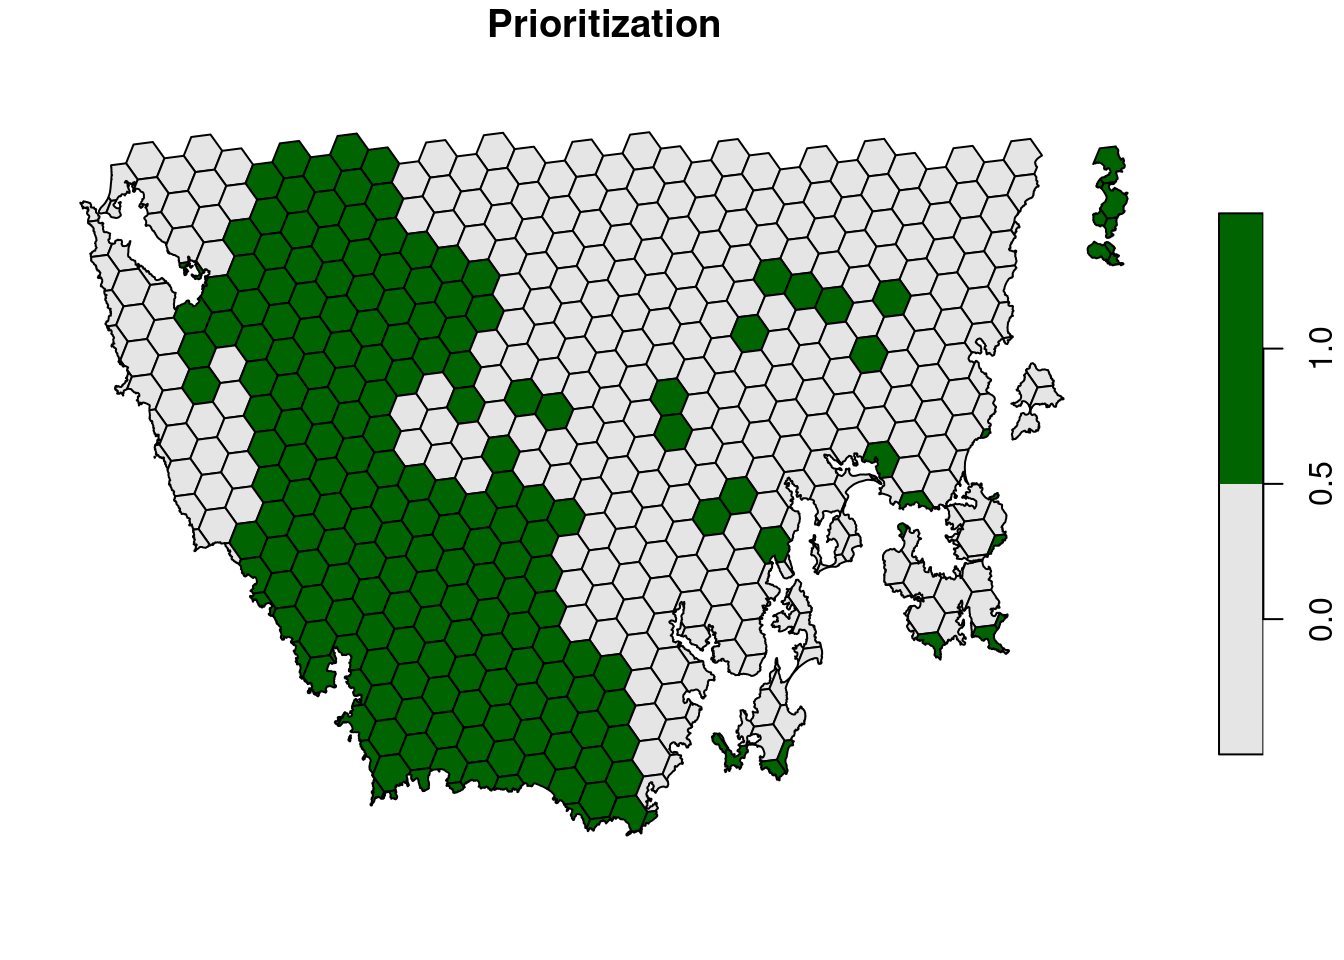
\includegraphics[width=0.65\linewidth]{prioritizr-workshop-manual_files/figure-latex/budget-weights-2} \end{center}

\begin{Shaded}
\begin{Highlighting}[]
\CommentTok{# calculate feature representation}
\NormalTok{r7 <-}\StringTok{ }\KeywordTok{eval_feature_representation_summary}\NormalTok{(p7, s7[, }\StringTok{"solution_1"}\NormalTok{])}
\end{Highlighting}
\end{Shaded}

\begin{verbatim}
## Warning: Support for sp package will be deprecated.
## i Use `sf::st_as_sf()` to convert data for future compatibility.
\end{verbatim}

\begin{Shaded}
\begin{Highlighting}[]
\CommentTok{# calculate number of features with targets met}
\KeywordTok{sum}\NormalTok{(r7}\OperatorTok{$}\NormalTok{relative_held }\OperatorTok{>=}\StringTok{ }\FloatTok{0.2}\NormalTok{, }\DataTypeTok{na.rm =} \OtherTok{TRUE}\NormalTok{)}
\end{Highlighting}
\end{Shaded}

\begin{verbatim}
## [1] 16
\end{verbatim}

\begin{Shaded}
\begin{Highlighting}[]
\CommentTok{# find out which features have their targets met when we add weights,}
\CommentTok{# note that NA is for vegetation.61}
\KeywordTok{print}\NormalTok{(r7}\OperatorTok{$}\NormalTok{feature[r7}\OperatorTok{$}\NormalTok{relative_held }\OperatorTok{>=}\StringTok{ }\FloatTok{0.2}\NormalTok{])}
\end{Highlighting}
\end{Shaded}

\begin{verbatim}
##  [1] "vegetation_1"  "vegetation_5"  "vegetation_14" "vegetation_17"
##  [5] "vegetation_18" "vegetation_19" "vegetation_20" "vegetation_21"
##  [9] "vegetation_22" "vegetation_23" "vegetation_24" "vegetation_25"
## [13] "vegetation_26" "vegetation_27" "vegetation_28" "vegetation_29"
\end{verbatim}

\begin{rmdquestion}
\begin{enumerate}
\def\labelenumi{\arabic{enumi}.}
\tightlist
\item
  What is the name of the feature with the smallest weight?
\item
  What is the cost of the sixth (\texttt{s6}) and seventh (\texttt{s7}) solutions?
\item
  Does there seem to be a big difference in which planning units were selected in the sixth (\texttt{s6}) and seventh (\texttt{s7}) solutions?
\item
  Is there a difference between which features are adequately represented in the sixth (\texttt{s6}) and seventh (\texttt{s7}) solutions? If so, what is the difference?
\end{enumerate}
\end{rmdquestion}

\hypertarget{solution-portfolios}{%
\section{Solution portfolios}\label{solution-portfolios}}

In systematic conservation planning, only rarely do we have data on all of the stakeholder preferences and biodiversity features that we are interested in conserving. As a consequence, it is often useful to generate a portfolio of near optimal solutions to present to decision makers to guide the reserve selection process. Generally we would want many solutions in our portfolio (e.g.~1000) to ensure that our portfolio contains a range of spatially distinct solutions, but here we will generate a portfolio containing just six near-optimal solutions so the code doesn't take too long to run. We will also increase the optimality gap to obtain solutions that are more suboptimal than earlier (the default gap value is 0.1).

\begin{Shaded}
\begin{Highlighting}[]
\CommentTok{# make problem with a shuffle portfolio}
\NormalTok{p8 <-}\StringTok{ }\KeywordTok{problem}\NormalTok{(pu_data, veg_data, }\DataTypeTok{cost_column =} \StringTok{"cost"}\NormalTok{) }\OperatorTok
\StringTok{      }\KeywordTok{add_max_features_objective}\NormalTok{(budget) }\OperatorTok
\StringTok{      }\KeywordTok{add_relative_targets}\NormalTok{(}\FloatTok{0.2}\NormalTok{) }\OperatorTok
\StringTok{      }\KeywordTok{add_feature_weights}\NormalTok{(wts) }\OperatorTok
\StringTok{      }\KeywordTok{add_binary_decisions}\NormalTok{() }\OperatorTok
\StringTok{      }\KeywordTok{add_shuffle_portfolio}\NormalTok{(}\DataTypeTok{number_solutions =} \DecValTok{6}\NormalTok{,}
                            \DataTypeTok{remove_duplicates =} \OtherTok{FALSE}\NormalTok{) }\OperatorTok
\StringTok{      }\KeywordTok{add_lpsymphony_solver}\NormalTok{(}\DataTypeTok{verbose =} \OtherTok{TRUE}\NormalTok{, }\DataTypeTok{gap =} \DecValTok{10}\NormalTok{)}
\end{Highlighting}
\end{Shaded}

\begin{verbatim}
## Warning: Support for sp package will be deprecated.
## i Use `sf::st_as_sf()` to convert data for future compatibility.
\end{verbatim}

\begin{verbatim}
## Warning: Support for raster package will be deprecated.
## i Use `terra::rast()` to convert data for future compatibility.
\end{verbatim}

\clearpage

\begin{Shaded}
\begin{Highlighting}[]
\CommentTok{# print problem}
\KeywordTok{print}\NormalTok{(p8)}
\end{Highlighting}
\end{Shaded}

\begin{verbatim}
## A conservation problem (<ConservationProblem>)
\end{verbatim}

\begin{verbatim}
## +@data
\end{verbatim}

\begin{verbatim}
## |+@features:    "vegetation_1", "vegetation_2", "vegetation_3", "vegetation_4" , ... (32 total)
\end{verbatim}

\begin{verbatim}
## |\@planning units:
\end{verbatim}

\begin{verbatim}
## | +@data:       <SpatialPolygonsDataFrame> (516 total)
\end{verbatim}

\begin{verbatim}
## | +@costs:      continuous values (between 3.5972 and 47.2383)
\end{verbatim}

\begin{verbatim}
## | +@extent:     348703.1831, 5167774.5993, 611932.4474, 5344516.4109 (xmin, ymin, xmax, ymax)
\end{verbatim}

\begin{verbatim}
## | \@CRS:        WGS 84 / UTM zone 55S
\end{verbatim}

\begin{verbatim}
## +@formulation
\end{verbatim}

\begin{verbatim}
## |+@objective:   maximum representation objective (`budget` = 6580.6397)
\end{verbatim}

\begin{verbatim}
## |+@penalties:
\end{verbatim}

\begin{verbatim}
## ||\@1:          feature weights (`weights` = asymmetric continuous values (non-zero values between 1 and 10))
\end{verbatim}

\begin{verbatim}
## |+@targets:     relative targets (between 0.2 and 0.2)
\end{verbatim}

\begin{verbatim}
## |+@constraints: none specified
\end{verbatim}

\begin{verbatim}
## |\@decisions:   binary decision
\end{verbatim}

\begin{verbatim}
## \@optimization
\end{verbatim}

\begin{verbatim}
##  +@portfolio:   shuffle portfolio (`number_solutions` = 6, ...)
\end{verbatim}

\begin{verbatim}
##  \@solver:      lpsymphony (`gap` = 10, `time_limit` = 2147483647, `first_feasible` = FALSE, ...)
\end{verbatim}

\begin{verbatim}
## # i Use `summary(...)` to see complete formulation.
\end{verbatim}

\begin{Shaded}
\begin{Highlighting}[]
\CommentTok{# solve problem}
\CommentTok{# note that this will contain six solutions since we added a portfolio}
\NormalTok{s8 <-}\StringTok{ }\KeywordTok{solve}\NormalTok{(p8)}

\CommentTok{# print solution}
\KeywordTok{print}\NormalTok{(s8)}
\end{Highlighting}
\end{Shaded}

\begin{verbatim}
## class       : SpatialPolygonsDataFrame 
## features    : 516 
## extent      : 348703.2, 611932.4, 5167775, 5344516  (xmin, xmax, ymin, ymax)
## crs         : +proj=utm +zone=55 +south +datum=WGS84 +units=m +no_defs 
## variables   : 12
## names       :   id,             cost, status, locked_in, locked_out, pa_status, solution_1, solution_2, solution_3, solution_4, solution_5, solution_6 
## min values  :  557, 3.59717531470679,      0,         0,          0,         0,          0,          0,          0,          0,          0,          0 
## max values  : 1130,  47.238336402701,      2,         1,          1,         1,          1,          1,          1,          1,          1,          1
\end{verbatim}

\begin{Shaded}
\begin{Highlighting}[]
\CommentTok{# calculate the cost of the first solution}
\KeywordTok{sum}\NormalTok{(s8}\OperatorTok{$}\NormalTok{solution_}\DecValTok{1} \OperatorTok{*}\StringTok{ }\NormalTok{s8}\OperatorTok{$}\NormalTok{cost)}
\end{Highlighting}
\end{Shaded}

\begin{verbatim}
## [1] 1188.274
\end{verbatim}

\begin{Shaded}
\begin{Highlighting}[]
\CommentTok{# calculate the cost of the second solution}
\KeywordTok{sum}\NormalTok{(s8}\OperatorTok{$}\NormalTok{solution_}\DecValTok{2} \OperatorTok{*}\StringTok{ }\NormalTok{s8}\OperatorTok{$}\NormalTok{cost)}
\end{Highlighting}
\end{Shaded}

\begin{verbatim}
## [1] 1214.064
\end{verbatim}

\begin{Shaded}
\begin{Highlighting}[]
\CommentTok{# calculate the proportion of planning units with the same solution values}
\CommentTok{# in the first and second solutions}
\KeywordTok{mean}\NormalTok{(s8}\OperatorTok{$}\NormalTok{solution_}\DecValTok{1} \OperatorTok{==}\StringTok{ }\NormalTok{s8}\OperatorTok{$}\NormalTok{solution_}\DecValTok{2}\NormalTok{)}
\end{Highlighting}
\end{Shaded}

\begin{verbatim}
## [1] 0.9825581
\end{verbatim}

\begin{Shaded}
\begin{Highlighting}[]
\CommentTok{# plot first solution}
\KeywordTok{spplot}\NormalTok{(s8, }\StringTok{"solution_1"}\NormalTok{, }\DataTypeTok{col.regions =} \KeywordTok{c}\NormalTok{(}\StringTok{"white"}\NormalTok{, }\StringTok{"darkgreen"}\NormalTok{),}
       \DataTypeTok{main =} \StringTok{"s8 (solution 1)"}\NormalTok{)}
\end{Highlighting}
\end{Shaded}

\begin{center}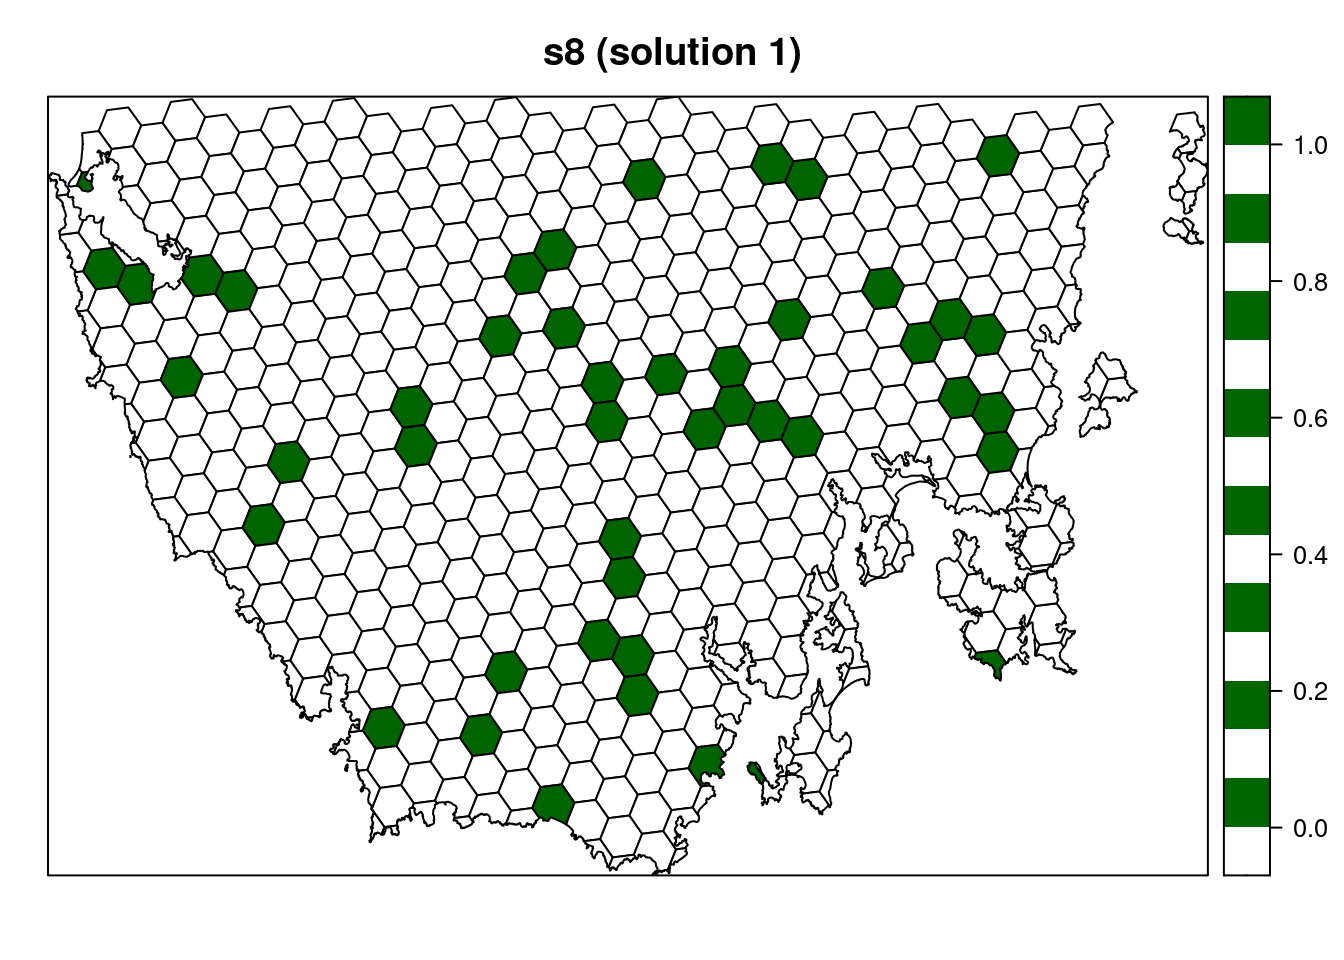
\includegraphics[width=0.65\linewidth]{prioritizr-workshop-manual_files/figure-latex/unnamed-chunk-47-1} \end{center}

\clearpage

\begin{Shaded}
\begin{Highlighting}[]
\CommentTok{# plot all solutions}
\NormalTok{s8_plots <-}\StringTok{ }\KeywordTok{lapply}\NormalTok{(}\KeywordTok{paste0}\NormalTok{(}\StringTok{"solution_"}\NormalTok{, }\KeywordTok{seq_len}\NormalTok{(}\DecValTok{6}\NormalTok{)), }\ControlFlowTok{function}\NormalTok{(x) \{}
  \KeywordTok{spplot}\NormalTok{(s8, x, }\DataTypeTok{main =}\NormalTok{ x, }\DataTypeTok{col.regions =} \KeywordTok{c}\NormalTok{(}\StringTok{"white"}\NormalTok{, }\StringTok{"darkgreen"}\NormalTok{))}
\NormalTok{\})}
\KeywordTok{do.call}\NormalTok{(grid.arrange, }\KeywordTok{append}\NormalTok{(s8_plots, }\KeywordTok{list}\NormalTok{(}\DataTypeTok{ncol =} \DecValTok{3}\NormalTok{)))}
\end{Highlighting}
\end{Shaded}

\begin{center}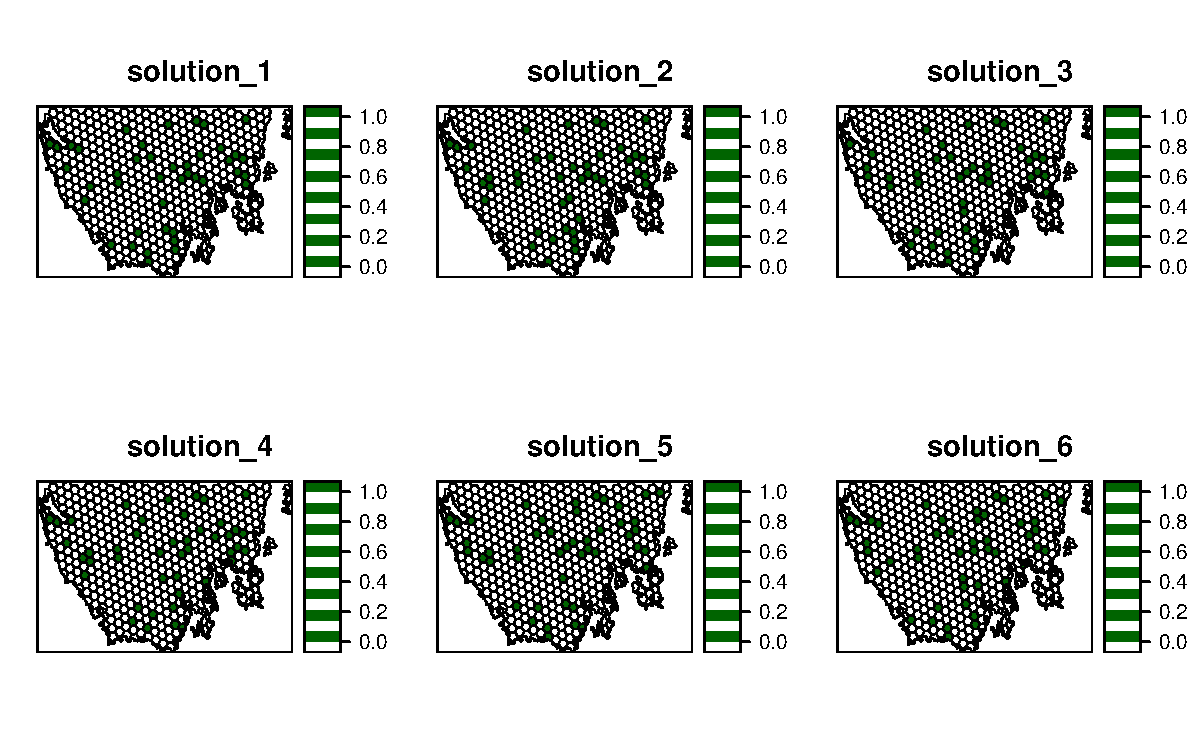
\includegraphics{prioritizr-workshop-manual_files/figure-latex/unnamed-chunk-48-1} \end{center}

\begin{rmdquestion}
\begin{enumerate}
\def\labelenumi{\arabic{enumi}.}
\tightlist
\item
  What is the cost of each of the six solutions in portfolio? Are their costs very different?
\item
  Are the solutions in the portfolio very different?
\item
  What could we do to obtain a portfolio with more different solutions?
\end{enumerate}
\end{rmdquestion}

\hypertarget{answers}{%
\chapter{Answers}\label{answers}}

This chapter contains the answers to the questions presented in the earlier chapters. The answers are provided here so you can check if your answers are correct.

\hypertarget{data-1}{%
\section{Data}\label{data-1}}

\hypertarget{planning-unit-data-1}{%
\subsection{Planning unit data}\label{planning-unit-data-1}}

\begin{rmdanswer}
\begin{enumerate}
\def\labelenumi{\arabic{enumi}.}
\tightlist
\item
  \texttt{nrow(pu\_data)}
\item
  \texttt{max(pu\_data\$cost)}
\item
  \texttt{sum(pu\_data\$locked\_in)}
\item
  \texttt{mean(pu\_data\$locked\_in)}
\item
  \texttt{sum(pu\_data\$locked\_out)}
\item
  \texttt{mean(pu\_data\$locked\_out)}
\item
  \texttt{assert\_that(min(c(pu\_data\$locked\_in,\ pu\_data\$locked\_out))\ ==\ 0)}
  \texttt{assert\_that(max(c(pu\_data\$locked\_in,\ pu\_data\$locked\_out))\ ==\ 1)}
\item
  \texttt{all(is.finite(pu\_data\$cost))}
\item
  \texttt{assert\_that(sum(duplicated(pu\_data\$id))\ ==\ 0)}
\item
  Yes, the eastern side of Tasmania is generally much cheaper than the western side.
\item
  Yes, most planning units covered by protected areas are located in the south-western side of Tasmania.
\end{enumerate}
\end{rmdanswer}

\clearpage

\hypertarget{vegetation-data-1}{%
\subsection{Vegetation data}\label{vegetation-data-1}}

\begin{rmdanswer}
\begin{enumerate}
\def\labelenumi{\arabic{enumi}.}
\tightlist
\item
  Central-north Tasmania
\item
  \texttt{cellStats(veg\_data{[}{[}12{]}{]},\ "mean")}
\item
  \texttt{names(veg\_data){[}which.max(cellStats(veg\_data,\ "sum")){]}}
\item
  Yes, they are the same.
\end{enumerate}
\end{rmdanswer}

\hypertarget{gap-analysis-1}{%
\section{Gap analysis}\label{gap-analysis-1}}

\hypertarget{feature-abundance-1}{%
\subsection{Feature abundance}\label{feature-abundance-1}}

\begin{rmdanswer}
\begin{enumerate}
\def\labelenumi{\arabic{enumi}.}
\tightlist
\item
  \texttt{median(abundance\_data\$absolute\_abundance\_km2)}
\item
  \texttt{min(abundance\_data\$absolute\_abundance\_km2)}
\item
  \texttt{abundance\_data\$feature{[}which.min(abundance\_data\$absolute\_abundance\_km2){]}}
\item
  \texttt{sum(abundance\_data\$absolute\_abundance\_km2)}
\item
  \texttt{sum(abundance\_data\$absolute\_abundance\_km2\ \textgreater{}\ set\_units(100,\ km\^{}2))}
\end{enumerate}
\end{rmdanswer}

\hypertarget{feature-representation-by-protected-areas-1}{%
\subsection{Feature representation by protected areas}\label{feature-representation-by-protected-areas-1}}

\begin{rmdanswer}
\begin{enumerate}
\def\labelenumi{\arabic{enumi}.}
\tightlist
\item
  \texttt{mean(repr\_data\$relative\_held,\ na.rm\ =\ TRUE)}
\item
  \texttt{mean(repr\_data\$absolute\_held\_km2,\ na.rm\ =\ TRUE)}
\item
  \texttt{repr\_data\$feature{[}which.max(repr\_data\$relative\_held){]}}
\item
  \texttt{repr\_data\$feature{[}which.max(repr\_data\$absolute\_held){]}}
\item
  No, just because a vegetation class is widespread does not necessarily mean that it has the greatest overlap with protected areas. In fact, due to biases in the establishment of protected areas this can often be the case.
\item
  Yes, the largest protected areas tend to have the great representation (broadly speaking). \newline
  \texttt{plot(abundance\_data\$absolute\_abundance,\ repr\_data\$relative\_held)}
\item
  \texttt{sum(repr\_data\$absolute\_held\ \textless{}\ 1e-10)} (floating point errors)
\item
  \texttt{sum(repr\_data\$relative\_held\ \textgreater{}\ 0.1,\ na.rm\ =\ TRUE)}
\item
  \texttt{sum(repr\_data\$relative\_held\ \textgreater{}\ 0.2,\ na.rm\ =\ TRUE)}
\end{enumerate}
\end{rmdanswer}

\hypertarget{spatial-prioritizations-1}{%
\section{Spatial prioritizations}\label{spatial-prioritizations-1}}

\hypertarget{starting-out-simple-1}{%
\subsection{Starting out simple}\label{starting-out-simple-1}}

\begin{rmdanswer}
\begin{enumerate}
\def\labelenumi{\arabic{enumi}.}
\tightlist
\item
  \texttt{sum(s1\$solution\_1)} \newline
  \texttt{mean(s1\$solution\_1)}
\item
  Yes, the planning units are generally spread out across most of the study area and they are not biased towards specific areas.
\item
  \texttt{all(feature\_representation(p1,\ s1{[},\ "solution\_1"{]})\$relative\_held\ \textgreater{}=\ 0.2)}
\end{enumerate}
\end{rmdanswer}

\hypertarget{adding-complexity-1}{%
\subsection{Adding complexity}\label{adding-complexity-1}}

\begin{rmdanswer}
\begin{enumerate}
\def\labelenumi{\arabic{enumi}.}
\tightlist
\item
  \texttt{sum(s2\$cost\ *\ s2\$solution\_1)} \newline
  \texttt{sum(s3\$cost\ *\ s3\$solution\_1)} \newline
  \texttt{sum(s4\$cost\ *\ s4\$solution\_1)}
\item
  \texttt{sum(s2\$solution\_1)} \newline
  \texttt{sum(s3\$solution\_1)} \newline
  \texttt{sum(s4\$solution\_1)}
\item
  No, just because a solution a solution has more planning units does not mean that it will cost less.
\item
  This is because the planning units covered by existing protected areas have a non-zero cost and locking in these planning units introduces inefficiencies into the solution. This is very common in real-world conservation prioritizations because existing protected areas are often in places that do little to benefit biodiversity \citep{r3}.
\item
  This is because some of the planning units that are highly degraded---based on just the planning unit costs and vegetation data---provide cost-efficient opportunities for meeting the targets and excluding them from the reserve selection process means that other more costly planning units are needed to meet the targets.
\item
  \texttt{sum(s4\$cost\ *\ s4\$solution\_1)\ -\ sum(s4\$cost\ *\ s4\$locked\_in)}
\item
  We get an error message stating the the problem is infeasible because there is no valid solution---even if we selected all the planning units the study area we would still not meet the targets.
\end{enumerate}
\end{rmdanswer}

\hypertarget{penalizing-fragmentation-1}{%
\subsection{Penalizing fragmentation}\label{penalizing-fragmentation-1}}

\begin{rmdanswer}
\begin{enumerate}
\def\labelenumi{\arabic{enumi}.}
\tightlist
\item
  The cost of the fourth solution is \texttt{sum(s4\$solution\_1\ *\ s4\$cost)} and the cost of the fifth solution is \texttt{sum(s5\$solution\_1\ *\ s5\$cost)}. The fifth solution (\texttt{s5}) costs more than the fourth solution (\texttt{s4}) because we have added penalties to the conservation planning problem to indicate that we are willing to accept a slightly more costly solution if it means that we can reduce fragmentation.
\item
  The solution is now nearly identical to the fourth solution (\texttt{s4}) and so has nearly the same cost. This penalty value is too low and is not useful because it does not reduce the fragmentation in our solution.
\item
  The solution now contains a lot of extra planning units that are not needed to meet our targets. In fact, nearly every planning unit in the study is now selected. This penalty value is too high and is not useful.
\end{enumerate}
\end{rmdanswer}

\hypertarget{budget-limited-prioritizations-1}{%
\subsection{Budget limited prioritizations}\label{budget-limited-prioritizations-1}}

\begin{rmdanswer}
\begin{enumerate}
\def\labelenumi{\arabic{enumi}.}
\tightlist
\item
  \texttt{names(veg\_data){[}which.min(wts){]}}
\item
  \texttt{sum(s6\$cost\ *\ s6\$solution\_1)} \newline
  \texttt{sum(s7\$cost\ *\ s7\$solution\_1)}
\item
  No, the sixth (\texttt{s6}) and seventh (\texttt{s7}) solutions both share many of the same selected planning units and there does not appear to be an obvious difference in the spatial location of the planning units which they do not share.
\item
  Yes. Both solutions contain adequately represent these features: \newline
  \texttt{r6\$feature{[}r6\$relative\_held\ \textgreater{}\ 0.2\ \&\ r7\$relative\_held\ \textgreater{}\ 0.2{]}} \newline
  The sixth (\texttt{s6}) is adequately represents these features too: \newline
  \texttt{r6\$feature{[}r6\$relative\_held\ \textgreater{}\ 0.2\ \&\ !r7\$relative\_held\ \textgreater{}\ 0.2{]}} \newline
  The seventh (\texttt{s7}) is adequately represents these features too: \newline
  \texttt{r7\$feature{[}r7\$relative\_held\ \textgreater{}\ 0.2\ \&\ !r6\$relative\_held\ \textgreater{}\ 0.2{]}}
\end{enumerate}
\end{rmdanswer}

\clearpage

\hypertarget{solution-portfolios-1}{%
\subsection{Solution portfolios}\label{solution-portfolios-1}}

\begin{rmdanswer}
\begin{enumerate}
\def\labelenumi{\arabic{enumi}.}
\tightlist
\item
  No the cost are very similar. \newline
  \texttt{sum(s8\$solution\_1\ *\ s8\$cost)} \newline
  \texttt{sum(s8\$solution\_2\ *\ s8\$cost)} \newline
  \texttt{sum(s8\$solution\_3\ *\ s8\$cost)} \newline
  \texttt{sum(s8\$solution\_4\ *\ s8\$cost)} \newline
  \texttt{sum(s8\$solution\_5\ *\ s8\$cost)} \newline
  \texttt{sum(s8\$solution\_6\ *\ s8\$cost)}
\item
  No the status of the planning units are very similar in the all of the solutions in the portfolio. \newline
  \texttt{mean((s8\$solution\_1\ ==\ s8\$solution\_2)\ \&\ (s8\$solution\_1\ ==\ s8\$solution\_3)\ \&\ \ (s8\$solution\_1\ ==\ s8\$solution\_4)\ \&\ (s8\$solution\_1\ ==\ s8\$solution\_5)\ \&\ \ (s8\$solution\_1\ ==\ s8\$solution\_6))}
\item
  We should increase the number of the solutions in the portfolio.
\end{enumerate}
\end{rmdanswer}

\hypertarget{acknowledgements}{%
\chapter{Acknowledgements}\label{acknowledgements}}

Many thanks to \href{https://icons8.com}{Icons8} for providing the icons used in this manual and to Yihui Xie for developing the \href{http://bookdown.org}{bookdown R package} that underpins this manual. We also thank Garrett Grolemund and Hadley Wickham for creating one of the Rstudio screenshots used in this manual that was originally a part of their \emph{R for Data Science} book.

\hypertarget{session-information}{%
\chapter{Session information}\label{session-information}}

\begin{Shaded}
\begin{Highlighting}[]
\CommentTok{# print session information}
\KeywordTok{sessionInfo}\NormalTok{()}
\end{Highlighting}
\end{Shaded}

\begin{verbatim}
## R version 4.2.3 (2023-03-15)
## Platform: x86_64-pc-linux-gnu (64-bit)
## Running under: Ubuntu 20.04.6 LTS
## 
## Matrix products: default
## BLAS:   /usr/lib/x86_64-linux-gnu/blas/libblas.so.3.9.0
## LAPACK: /usr/lib/x86_64-linux-gnu/lapack/liblapack.so.3.9.0
## 
## locale:
##  [1] LC_CTYPE=C.UTF-8       LC_NUMERIC=C           LC_TIME=C.UTF-8       
##  [4] LC_COLLATE=C.UTF-8     LC_MONETARY=C.UTF-8    LC_MESSAGES=C.UTF-8   
##  [7] LC_PAPER=C.UTF-8       LC_NAME=C              LC_ADDRESS=C          
## [10] LC_TELEPHONE=C         LC_MEASUREMENT=C.UTF-8 LC_IDENTIFICATION=C   
## 
## attached base packages:
## [1] stats     graphics  grDevices utils     datasets  methods   base     
## 
## other attached packages:
##  [1] gridExtra_2.3    assertthat_0.2.1 scales_1.2.1     units_0.8-1     
##  [5] mapview_2.11.0   rgeos_0.6-2      raster_3.6-20    rgdal_1.6-5     
##  [9] sp_1.6-0         prioritizr_8.0.0 lubridate_1.9.2  forcats_1.0.0   
## [13] stringr_1.5.0    dplyr_1.1.0      purrr_1.0.1      readr_2.1.4     
## [17] tidyr_1.3.0      tibble_3.2.1     ggplot2_3.4.1    tidyverse_2.0.0 
## 
## loaded via a namespace (and not attached):
##  [1] Rcpp_1.0.10         gurobi_10.0-1       ape_5.7-1          
##  [4] lattice_0.20-45     png_0.1-8           class_7.3-21       
##  [7] digest_0.6.31       utf8_1.2.3          slam_0.1-50        
## [10] R6_2.5.1            stats4_4.2.3        evaluate_0.20      
## [13] e1071_1.7-13        pillar_1.9.0        rlang_1.1.0        
## [16] rstudioapi_0.14     Matrix_1.5-3        rmarkdown_2.20     
## [19] exactextractr_0.9.1 webshot_0.5.4       htmlwidgets_1.6.1  
## [22] munsell_0.5.0       proxy_0.4-27        compiler_4.2.3     
## [25] xfun_0.37           pkgconfig_2.0.3     base64enc_0.1-3    
## [28] htmltools_0.5.4     tidyselect_1.2.0    bookdown_0.33      
## [31] codetools_0.2-19    fansi_1.0.4         tzdb_0.3.0         
## [34] withr_2.5.0         sf_1.0-12           grid_4.2.3         
## [37] satellite_1.0.4     nlme_3.1-162        gtable_0.3.1       
## [40] lifecycle_1.0.3     DBI_1.1.3           magrittr_2.0.3     
## [43] KernSmooth_2.23-20  cli_3.6.1           stringi_1.7.12     
## [46] leaflet_2.1.1       lpsymphony_1.26.3   ellipsis_0.3.2     
## [49] generics_0.1.3      vctrs_0.6.1         tools_4.2.3        
## [52] leafem_0.2.0        glue_1.6.2          hms_1.1.2          
## [55] crosstalk_1.2.0     parallel_4.2.3      fastmap_1.1.1      
## [58] yaml_2.3.7          timechange_0.2.0    colorspace_2.1-0   
## [61] terra_1.7-18        classInt_0.4-9      knitr_1.42
\end{verbatim}

\hypertarget{references}{%
\chapter{References}\label{references}}

\bibliography{references.bib}

\end{document}
